\chapter{بخش سوم}
 در این بخش برای سیستم بر اساس روش‌های درس داده شده کنترل‌کننده طراحی شده است که ادامه آورده شده است.
 \newpage
\begin{itemize}
	\item \lr{ziegler nichols}
	\begin{figure}[H]
		\centering
		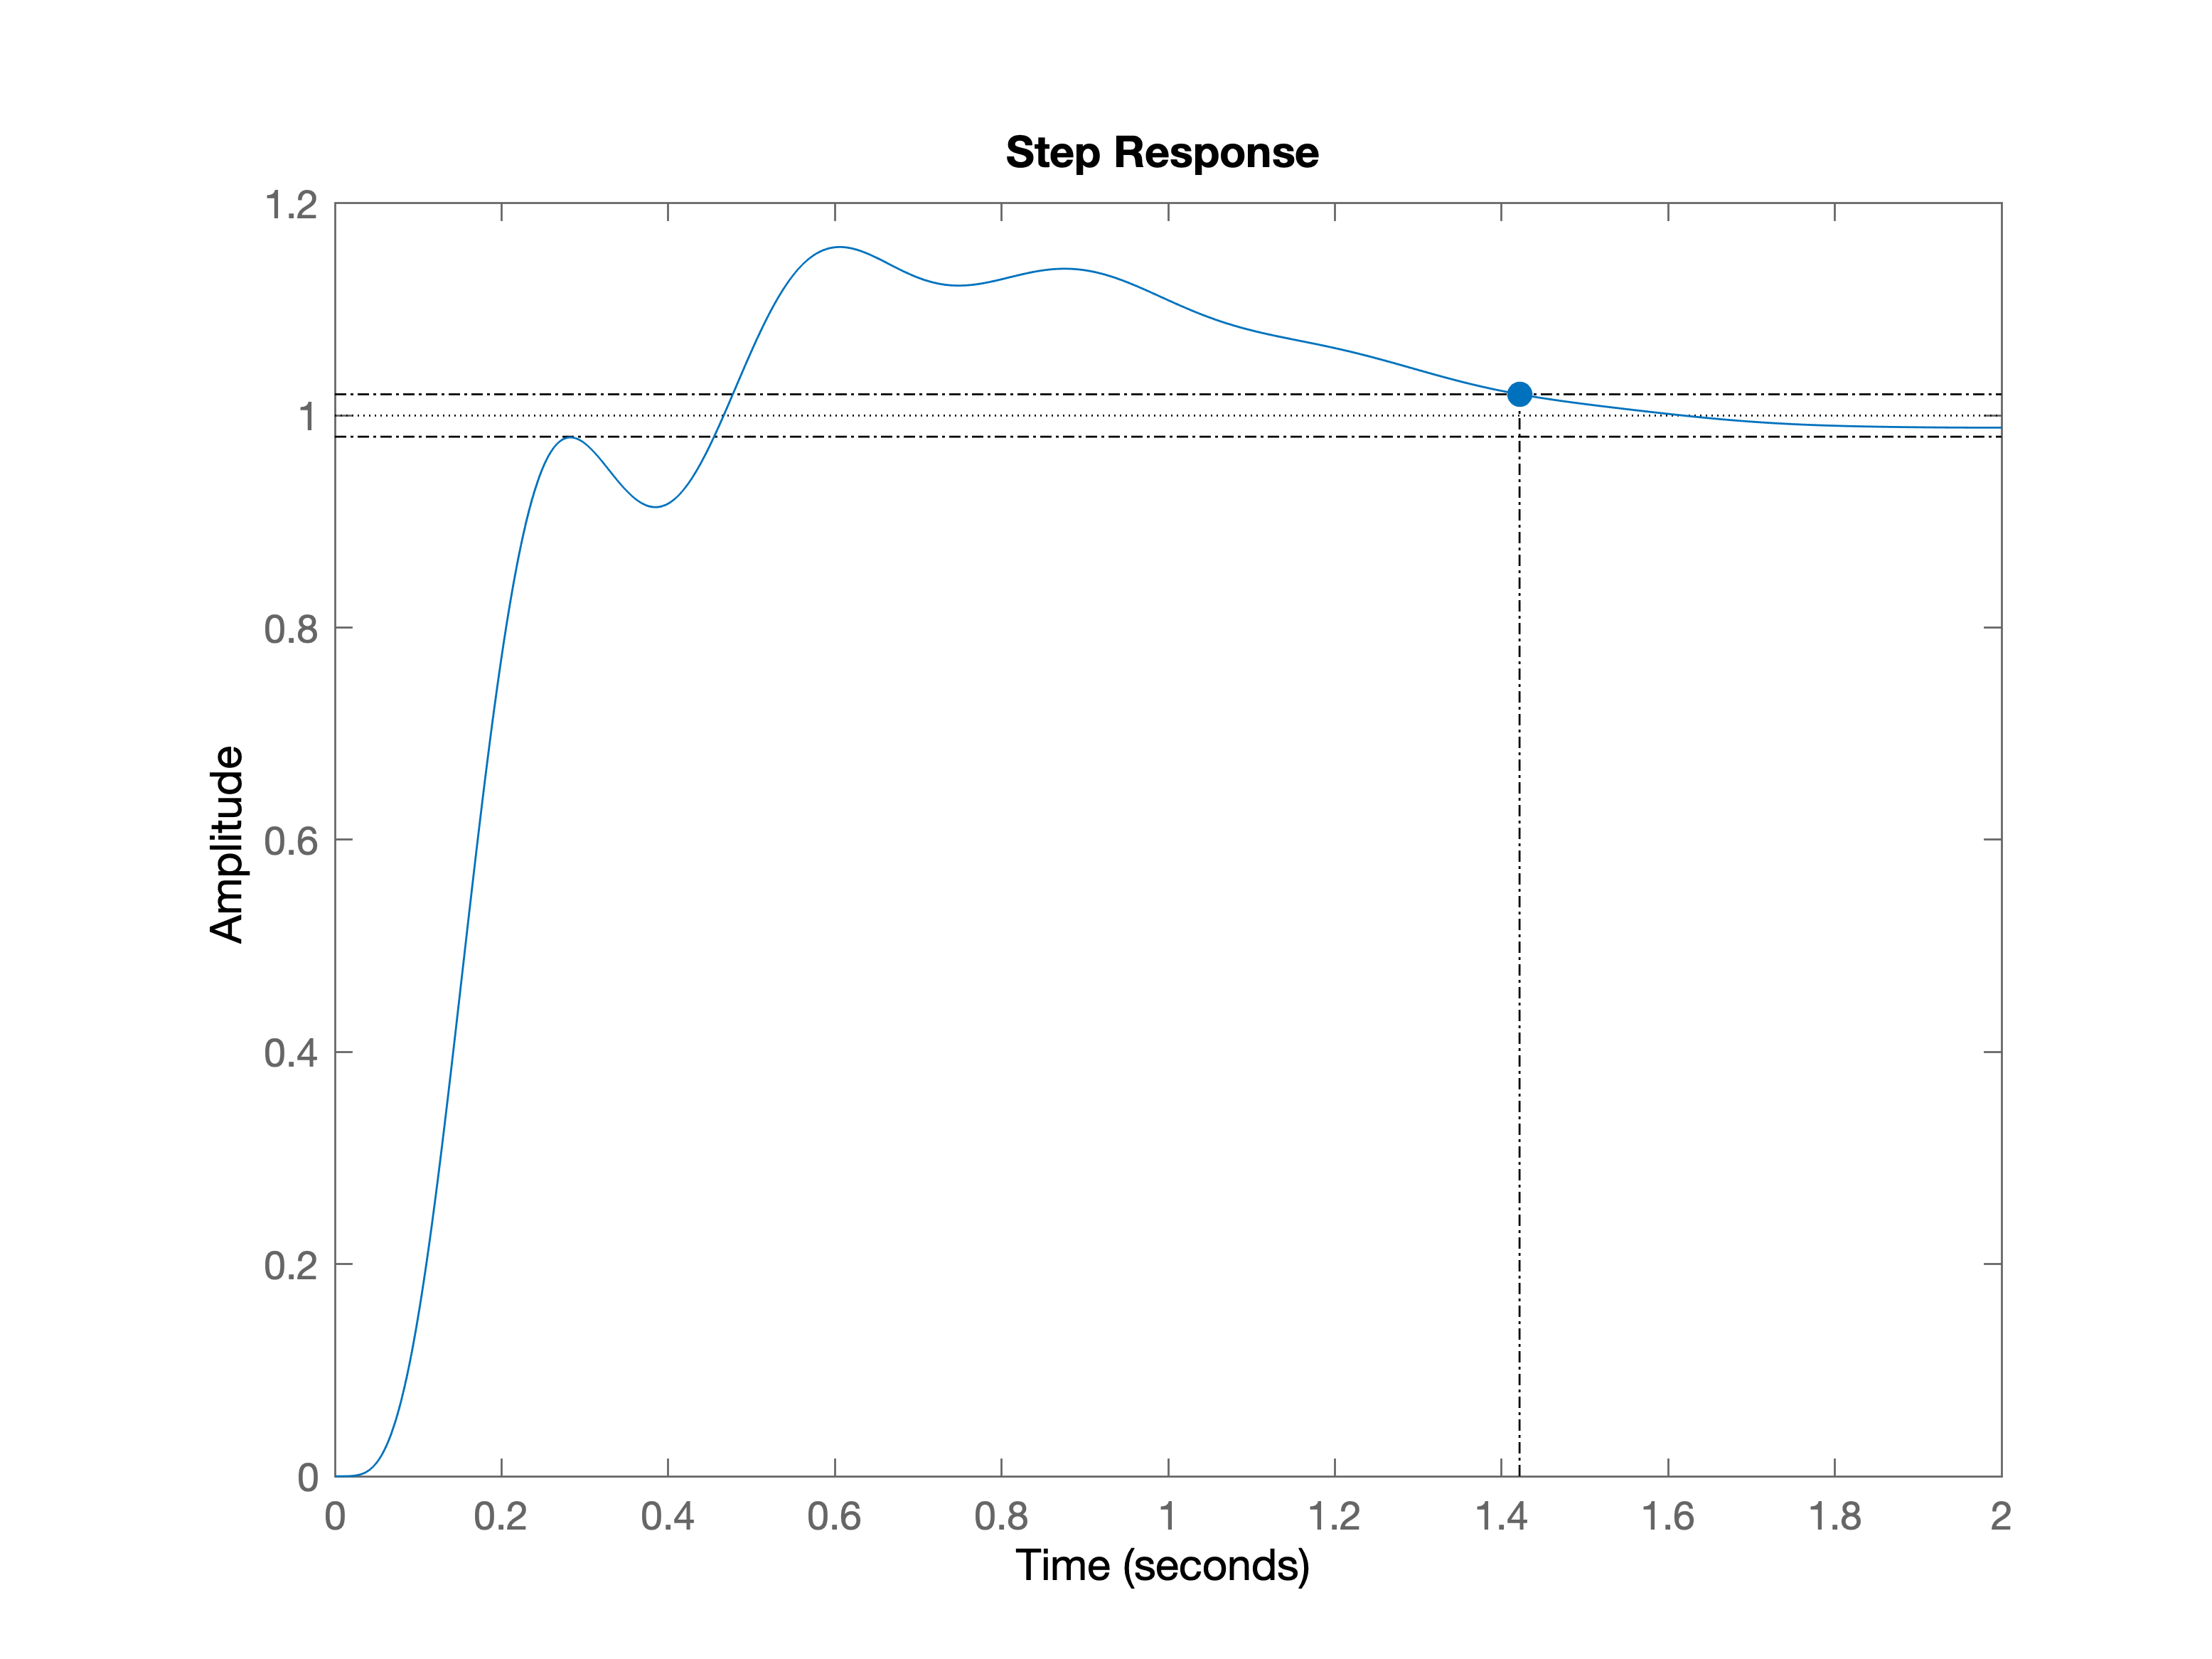
\includegraphics[width=12cm]{../Figure/P_III/zn.png}
		\caption{پاسخ پله سیستم در حضور کنترل‌کننده PID طراحی شده \lr{ziegler nichols}}
	\end{figure}
	\item \lr{refined ziegler nichols}
	\begin{figure}[H]
		\centering
		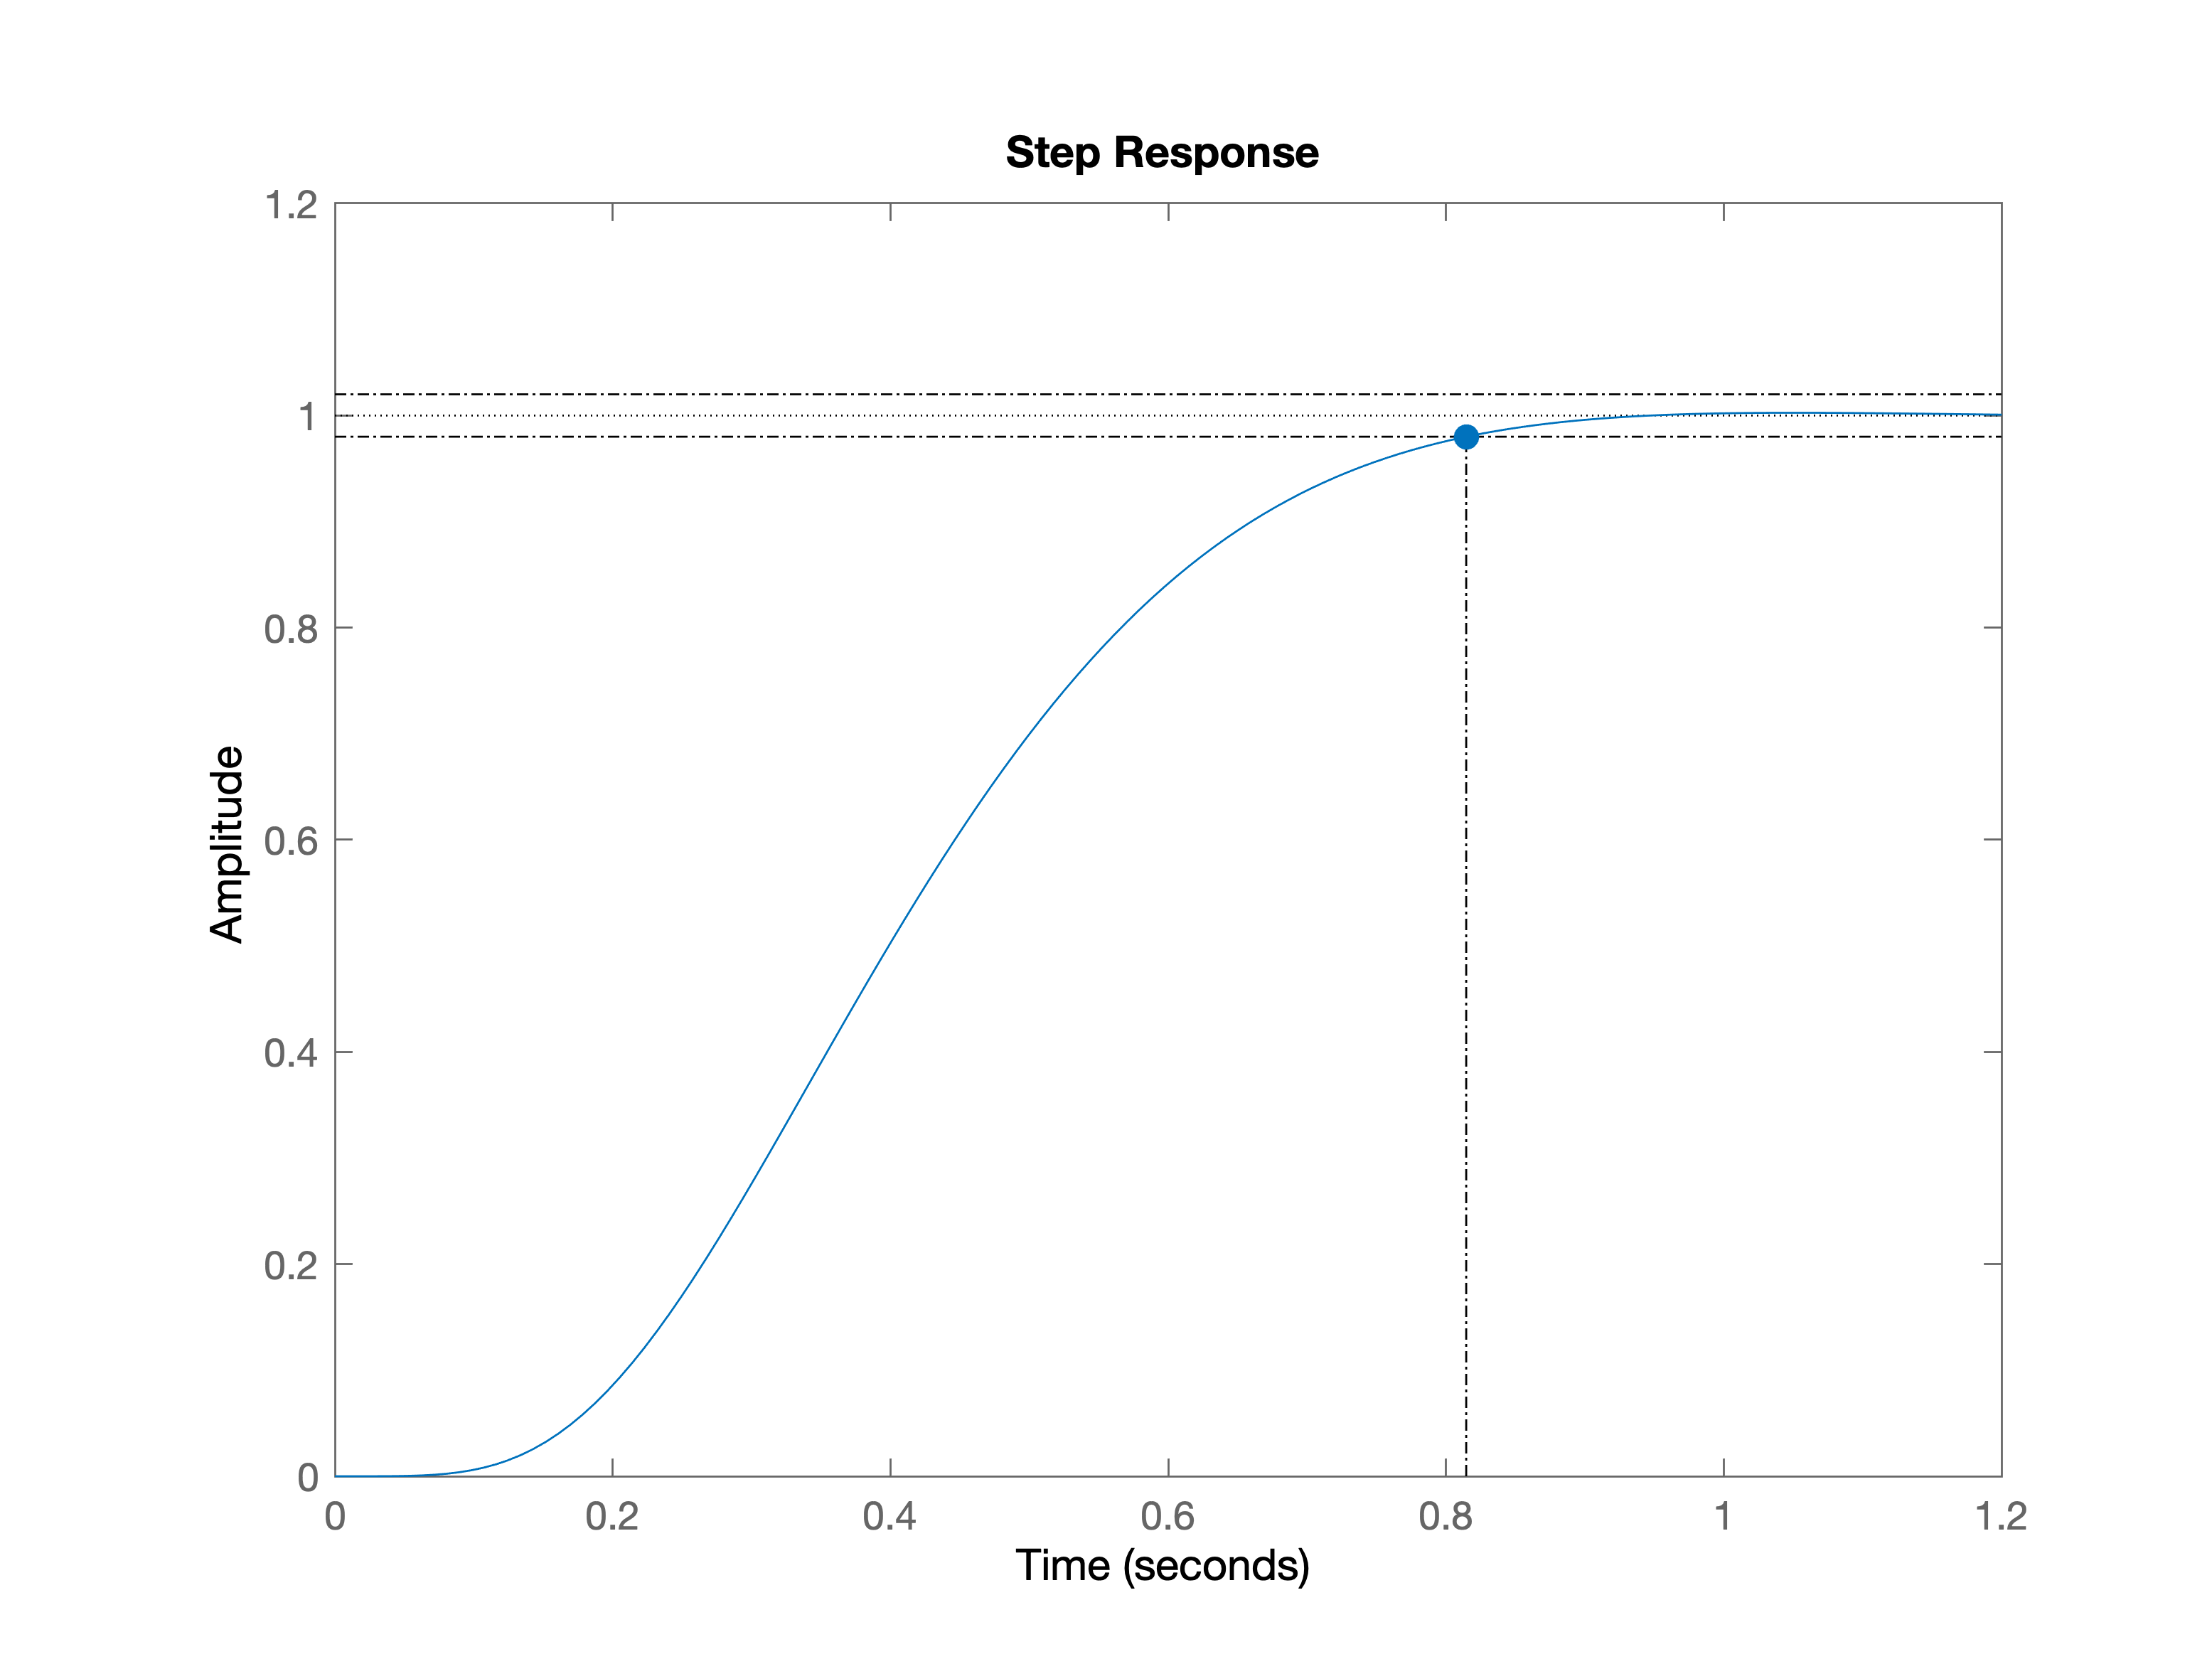
\includegraphics[width=12cm]{../Figure/P_III/rzn.png}
		\caption{پاسخ پله سیستم در حضور کنترل‌کننده PID طراحی شده \lr{refined ziegler nichol}}
	\end{figure}
	\item \lr{modified ziegler nichols}
	\begin{figure}[H]
		\centering
		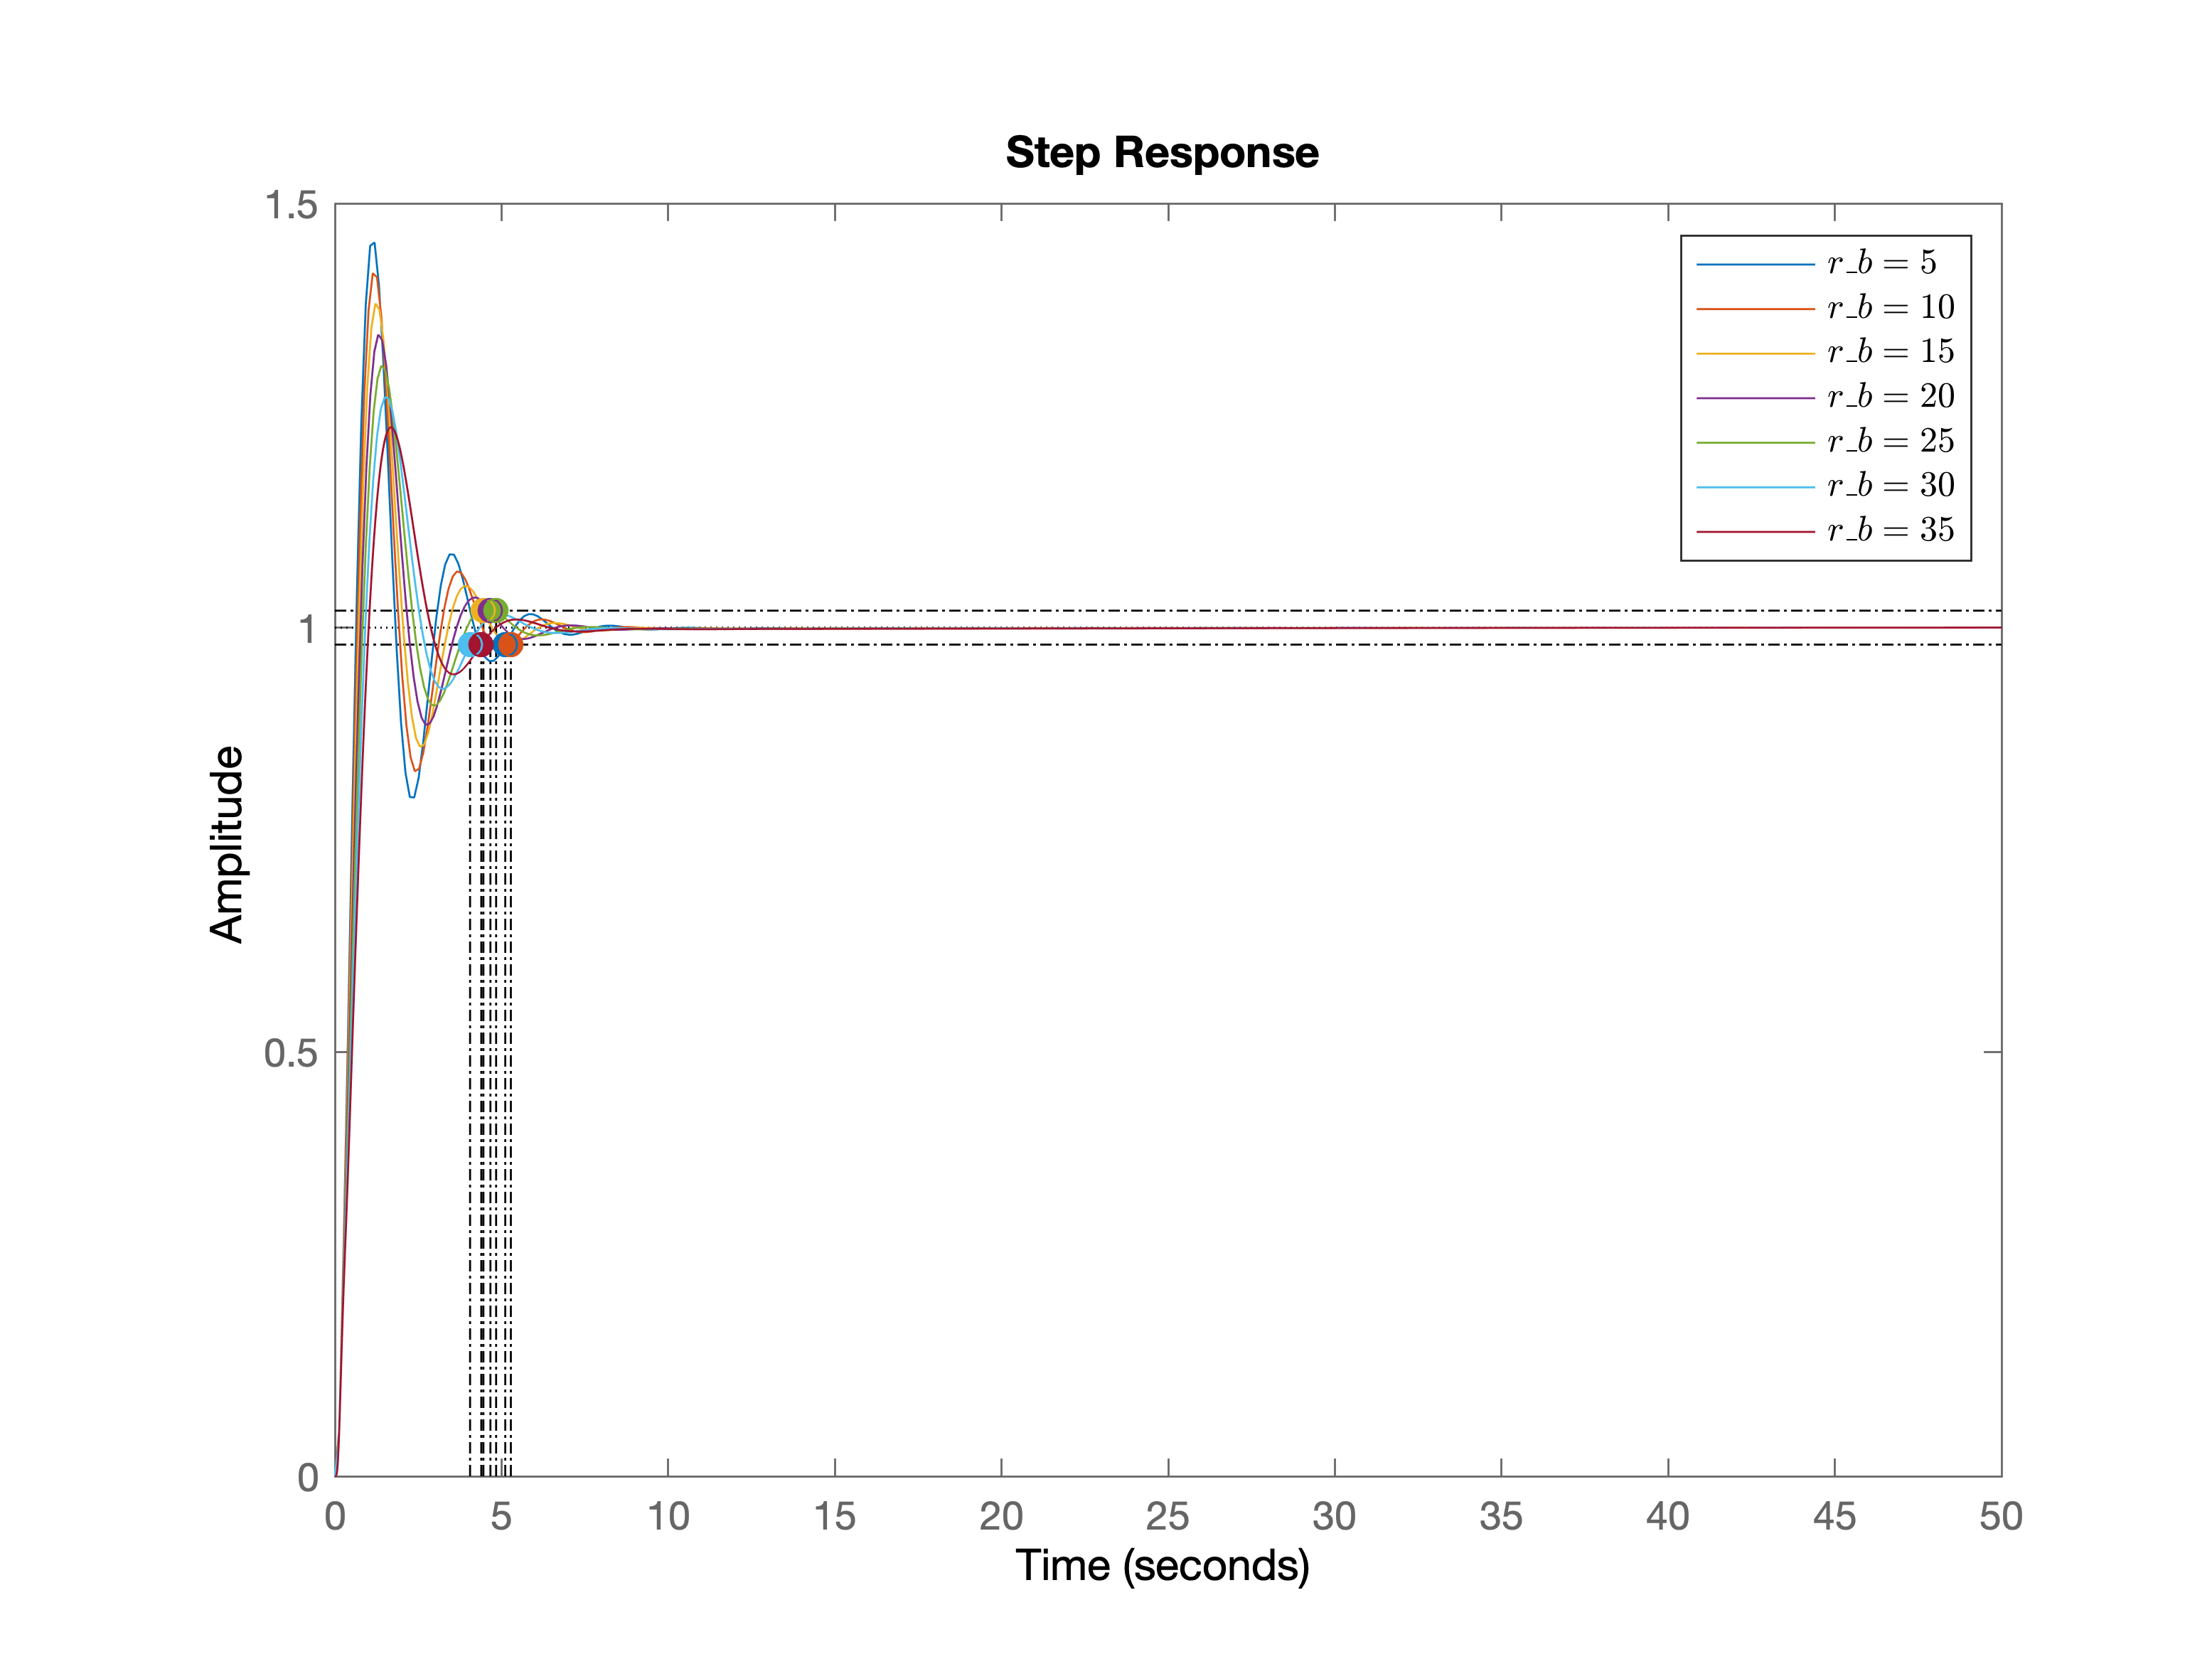
\includegraphics[width=12cm]{../Figure/P_III/mzn.png}
		\caption{پاسخ پله سیستم در حضور کنترل‌کننده PID طراحی شده \lr{modified ziegler nicholsl}}
	\end{figure}
	\item \lr{Cohen Coon}
	
	\begin{figure}[H]
		\centering
		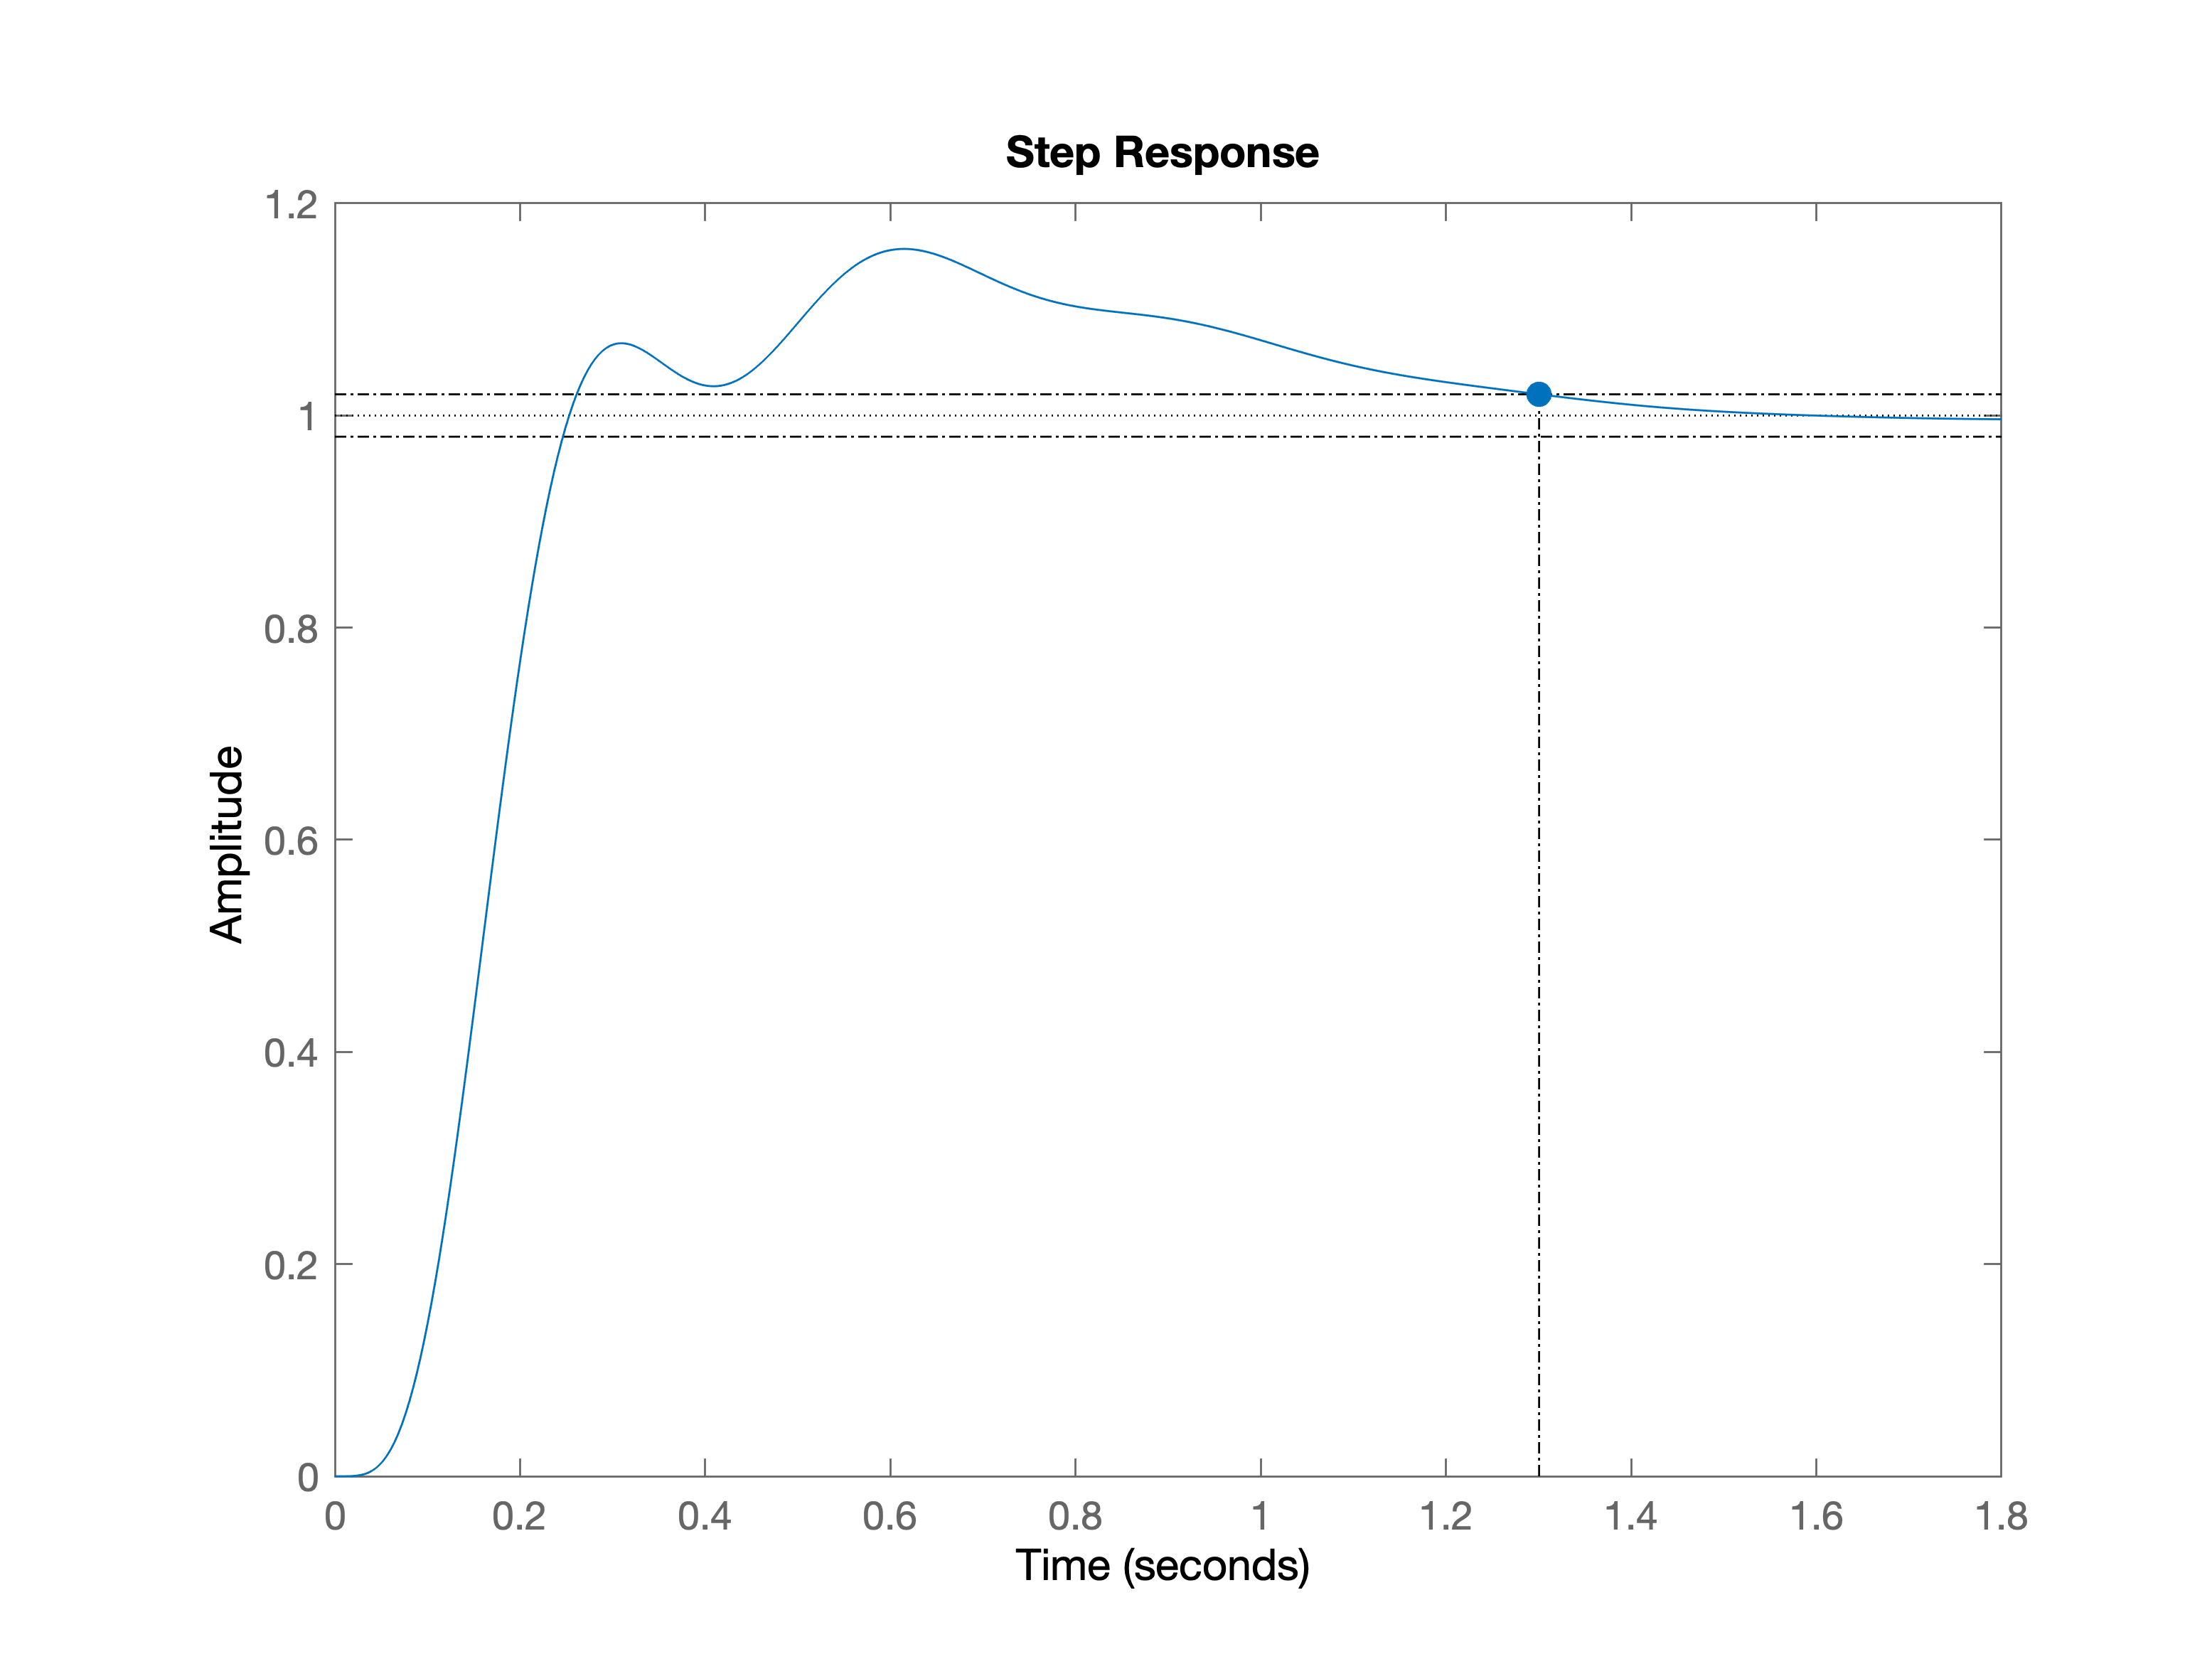
\includegraphics[width=12cm]{../Figure/P_III/cc.png}
		\caption{پاسخ پله سیستم در حضور کنترل‌کننده PID طراحی شده \lr{Cohen Coon}}
	\end{figure}
	\item \lr{Cohen Coon revisited}
	\begin{figure}[H]
		\centering
		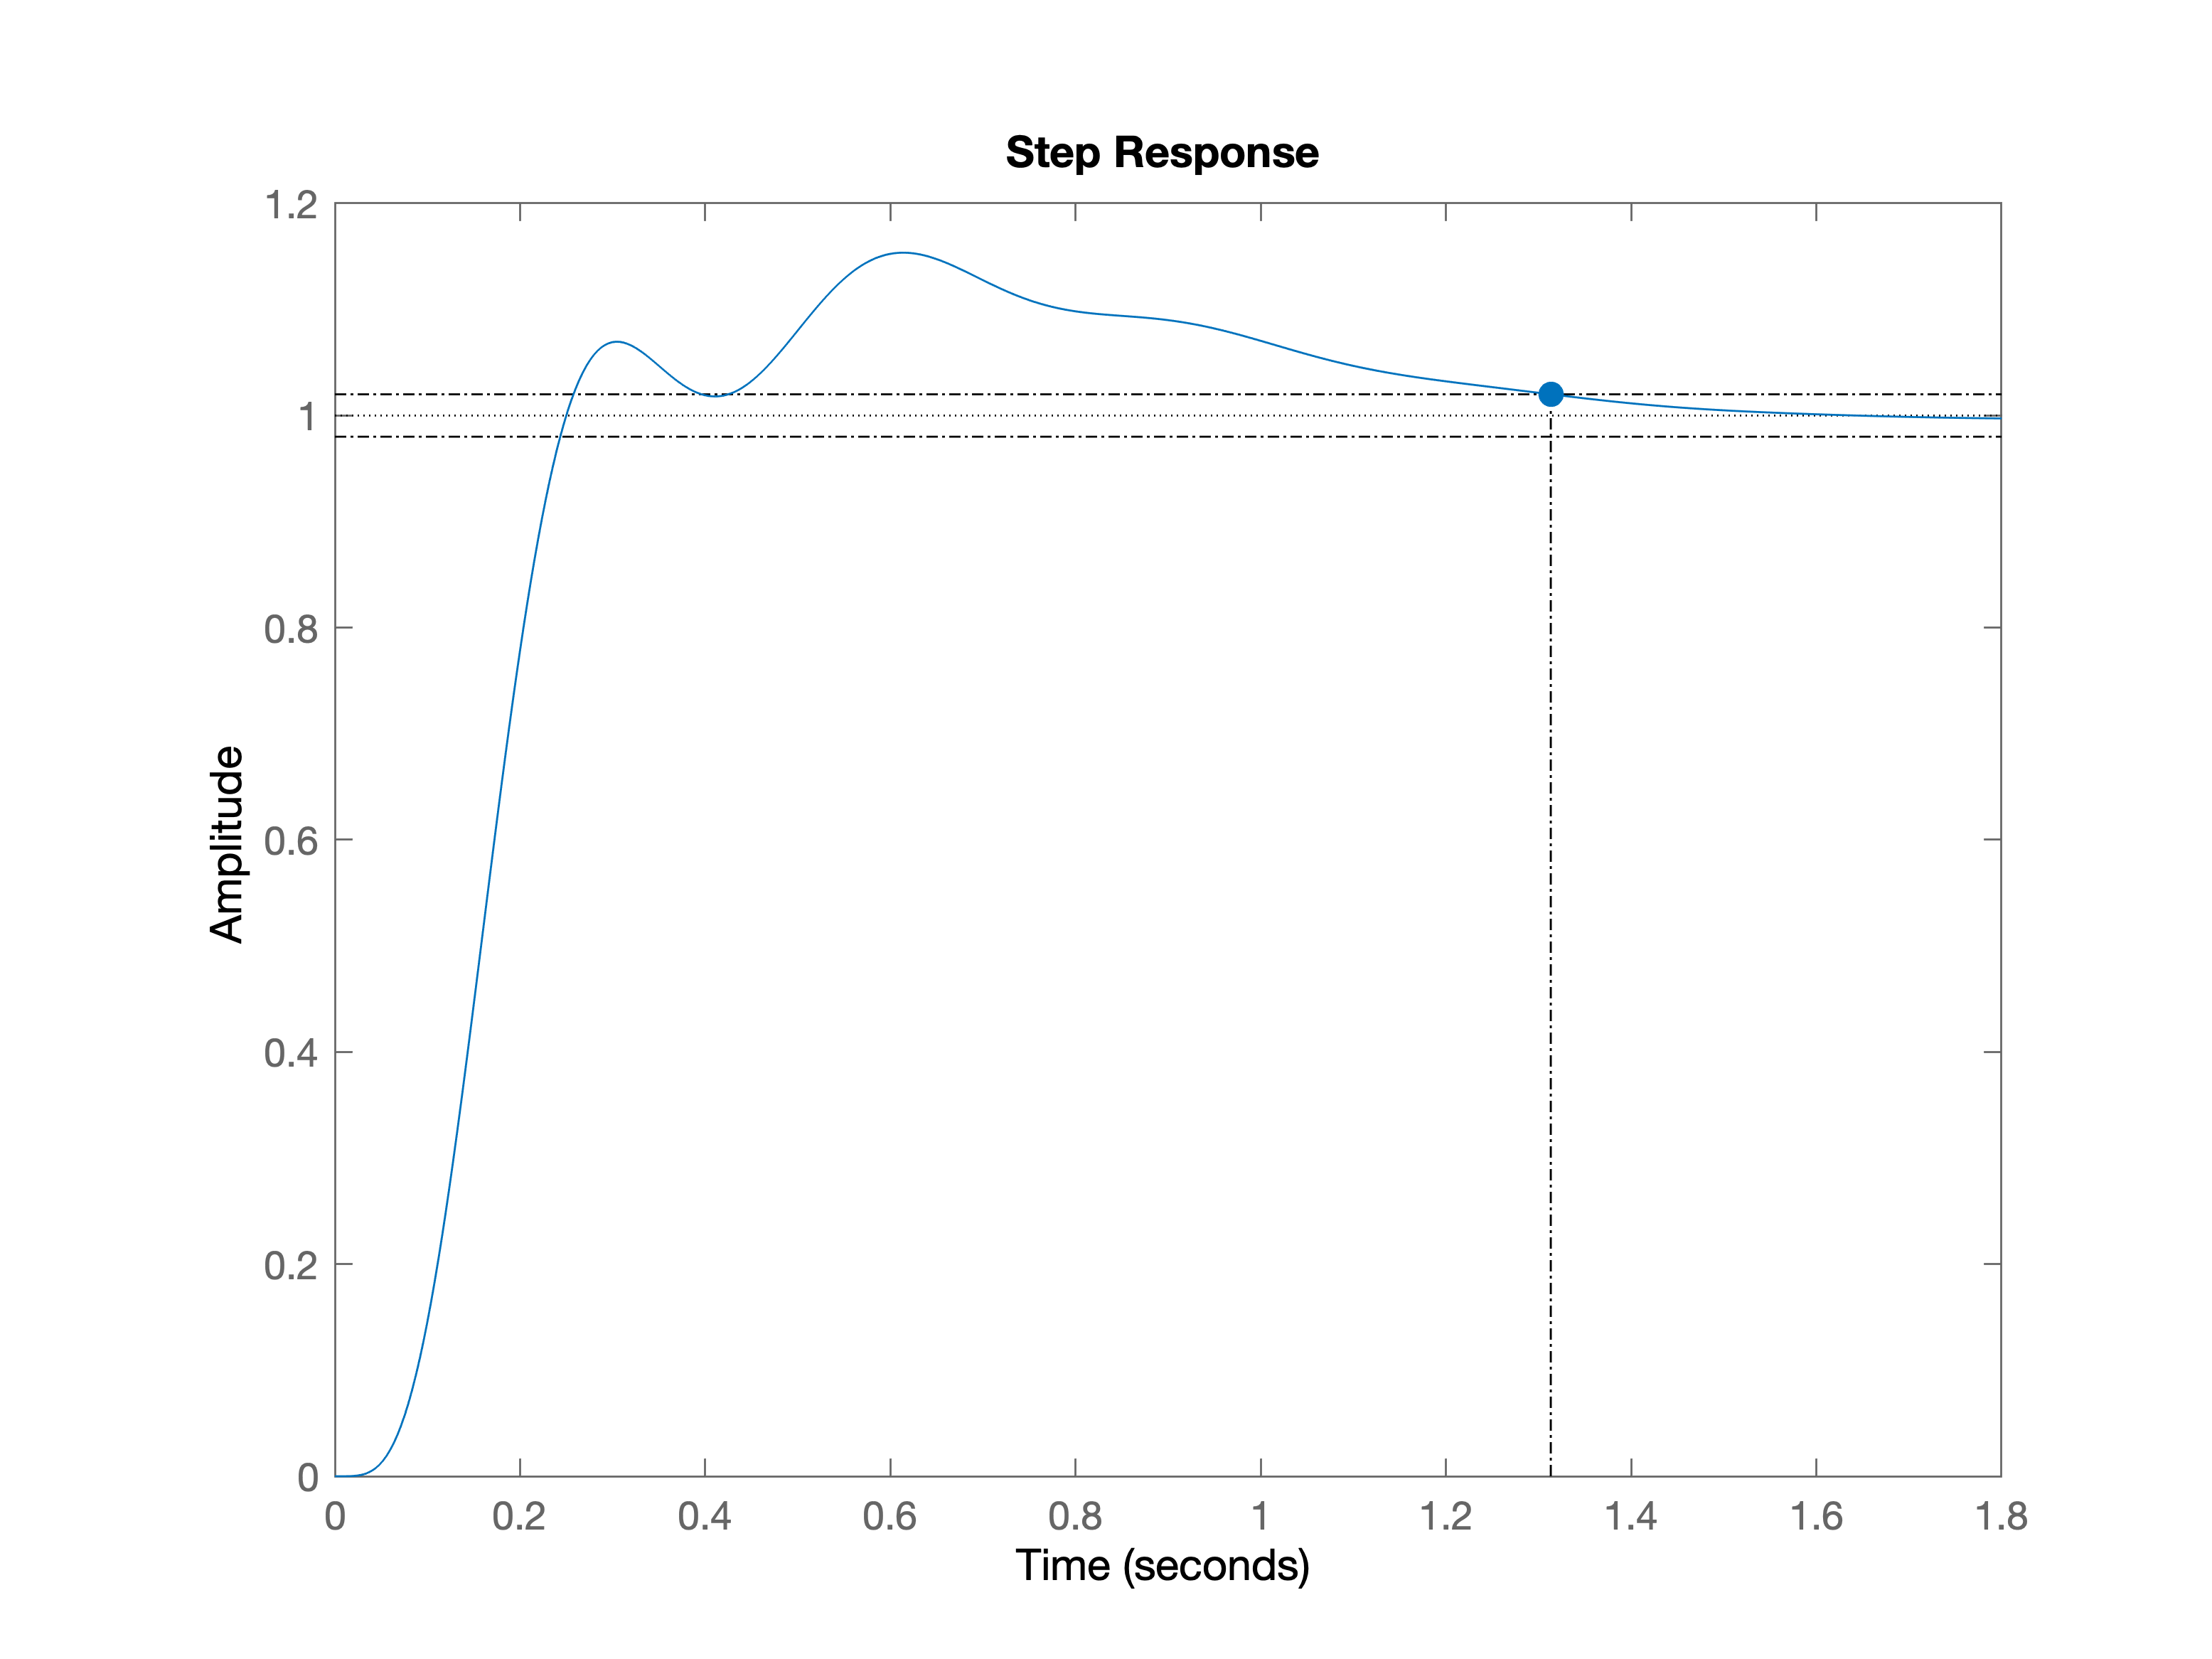
\includegraphics[width=12cm]{../Figure/P_III/ccr.png}
		\caption{پاسخ پله سیستم در حضور کنترل‌کننده PID طراحی شده \lr{Cohen Coon revisited}}
	\end{figure} 
	\item \lr{Astrom Hagglund}
	
	\begin{figure}[H]
		\centering
		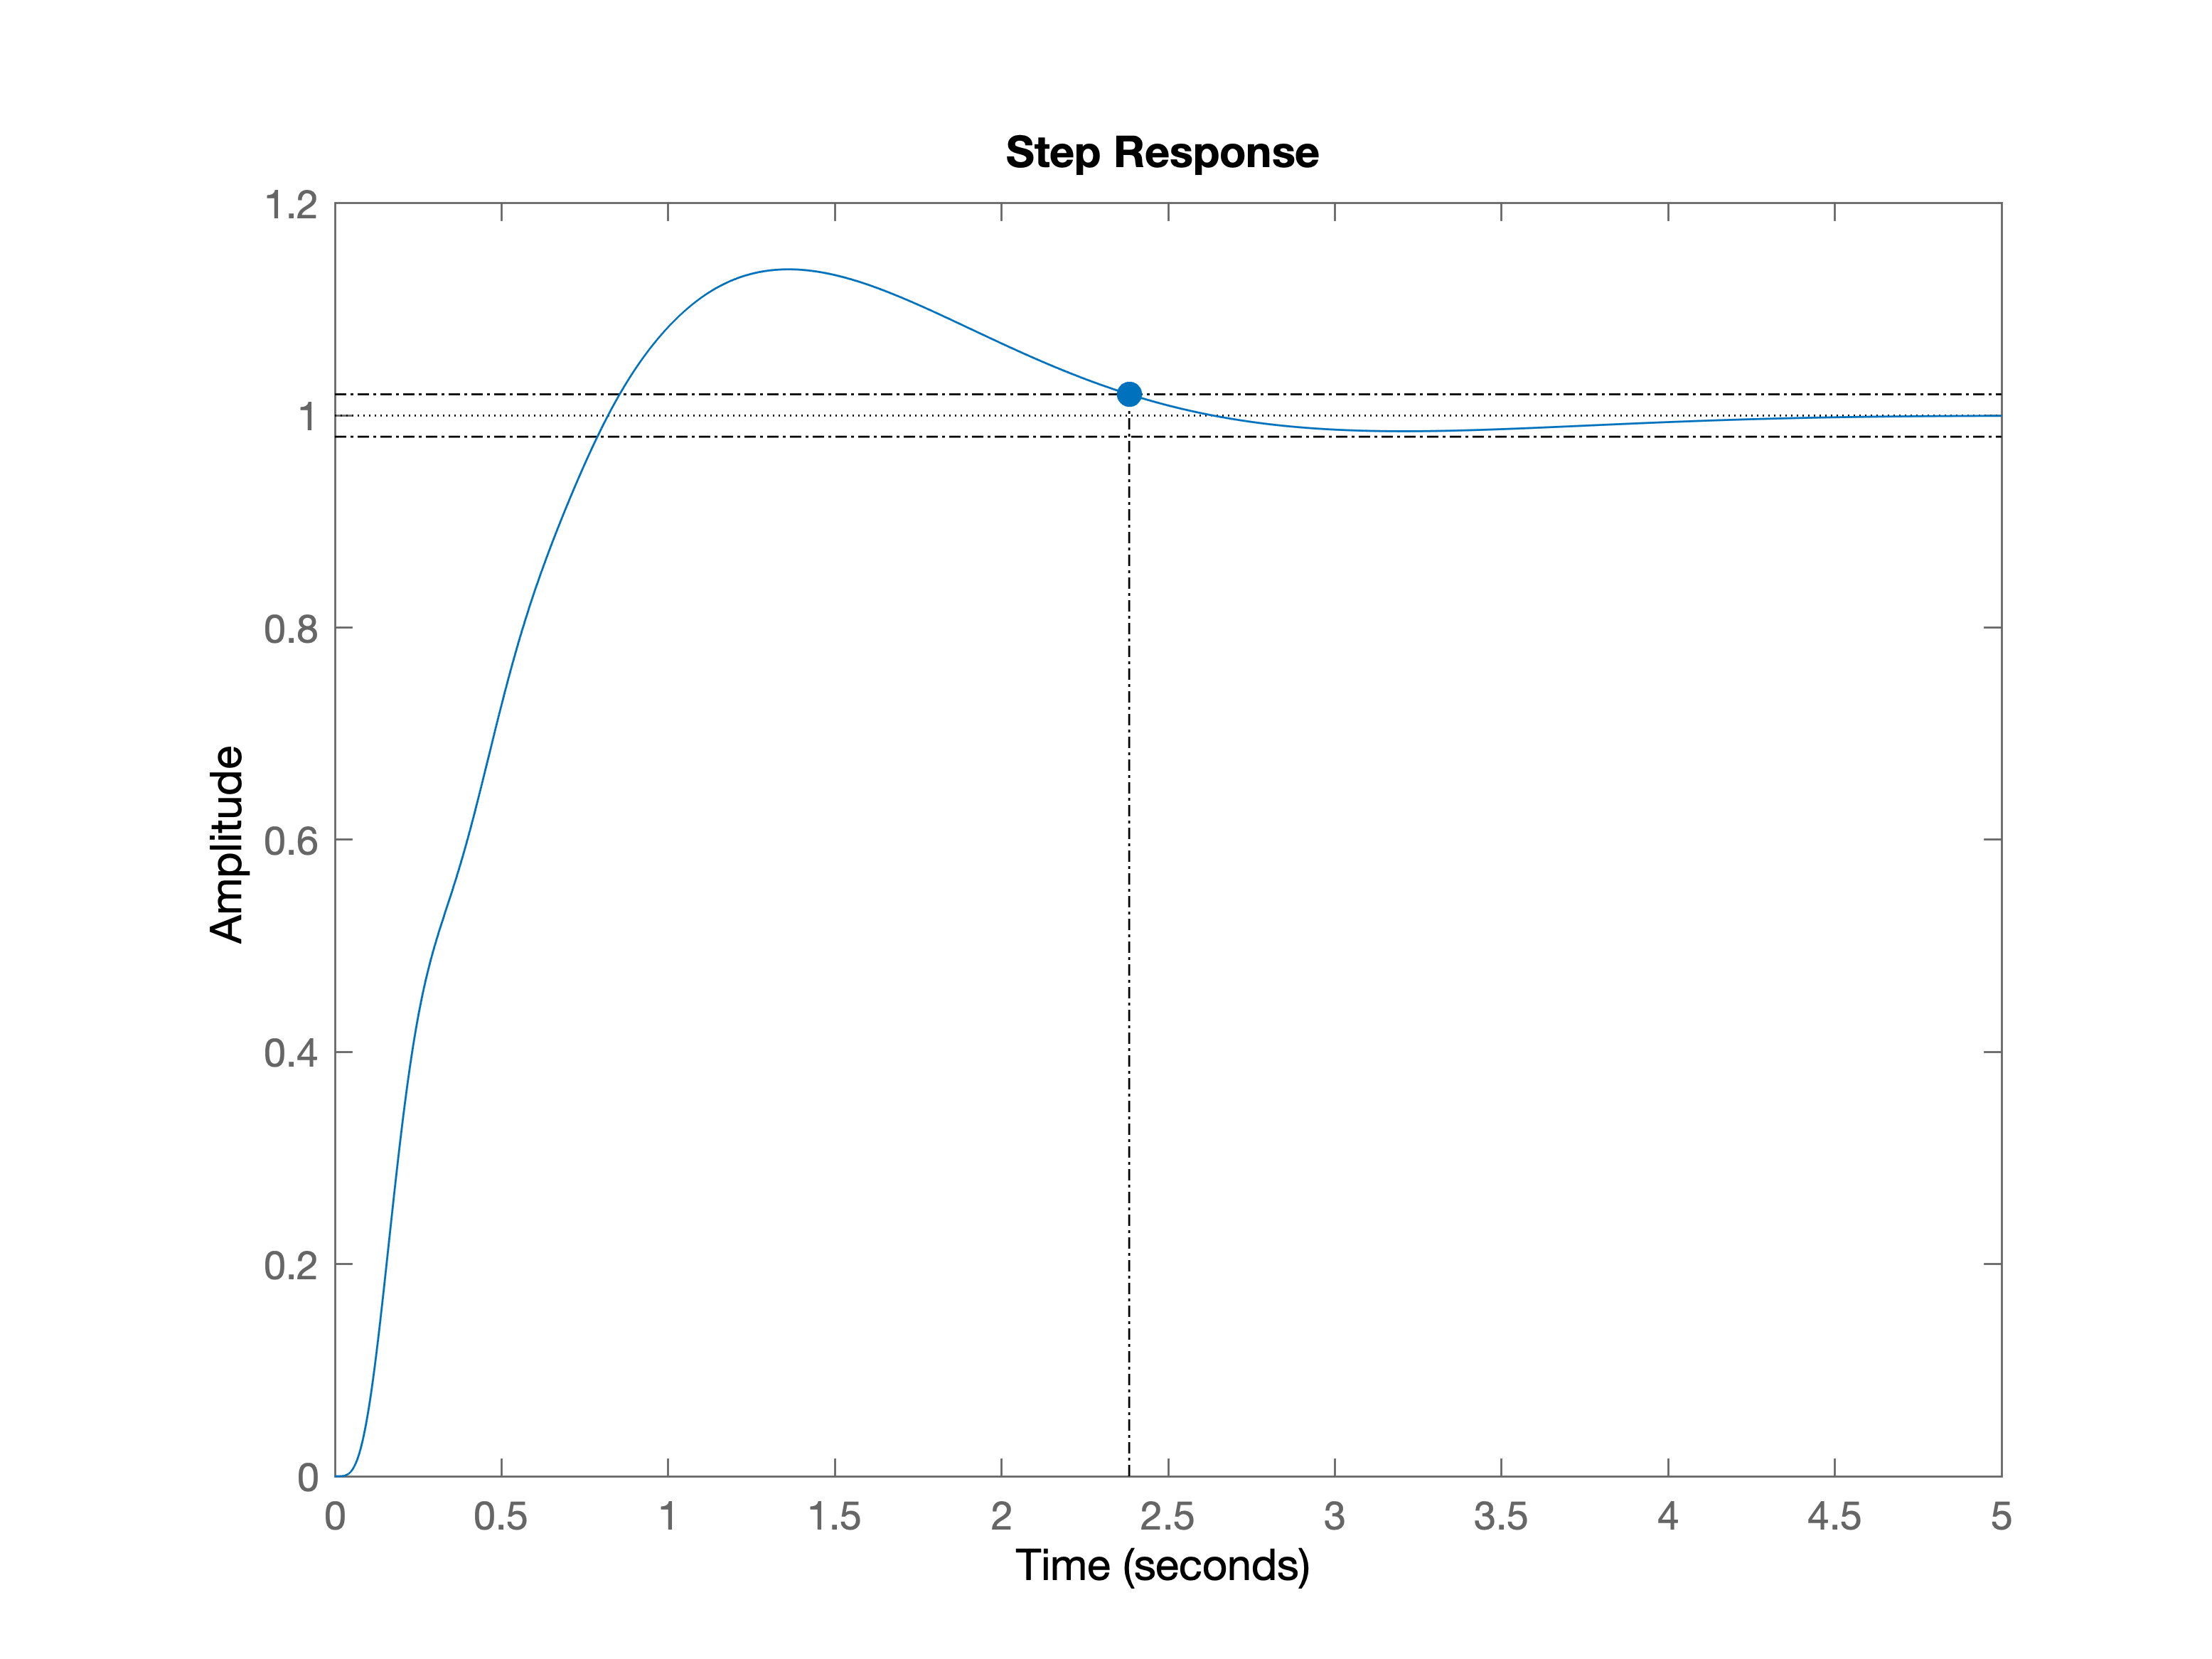
\includegraphics[width=12cm]{../Figure/P_III/ah.png}
		\caption{پاسخ پله سیستم در حضور کنترل‌کننده PID طراحی شده \lr{Astrom Hagglund}}
	\end{figure}  
	\item \lr{Frequency based Astrom Hagglund}
	
	\begin{figure}[H]
		\centering
		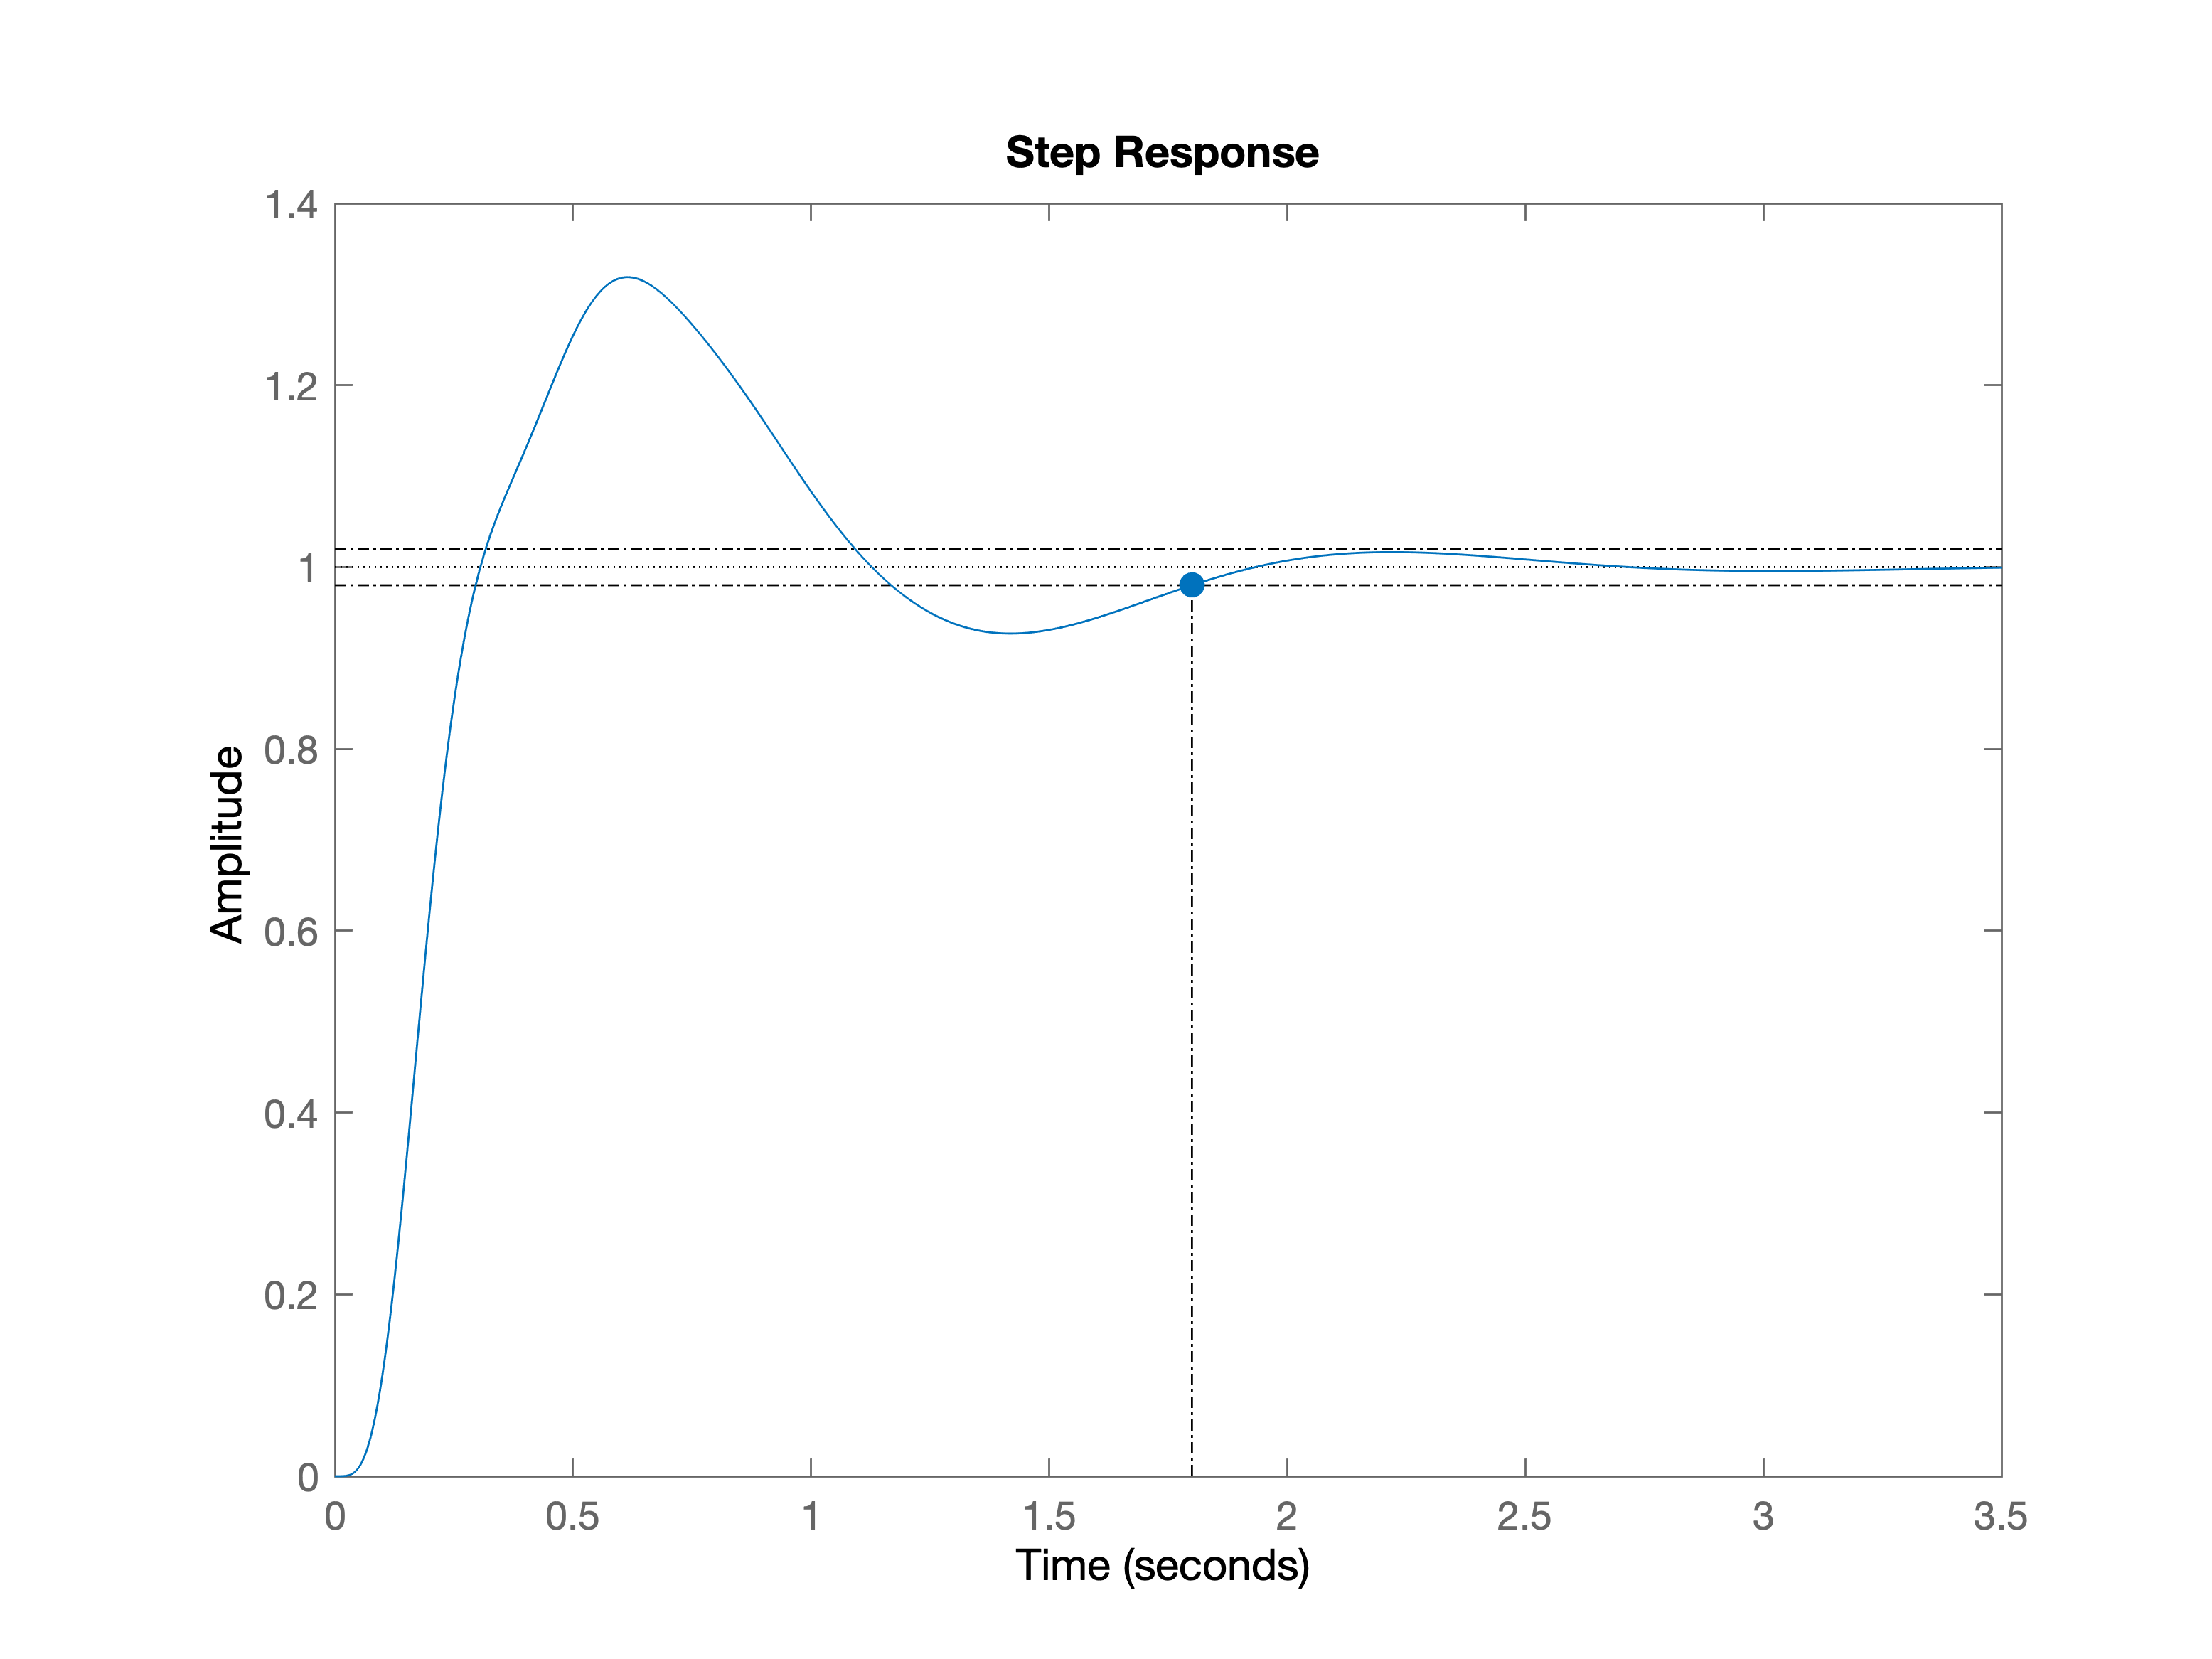
\includegraphics[width=12cm]{../Figure/P_III/fah.png}
		\caption{پاسخ پله سیستم در حضور کنترل‌کننده PID طراحی شده \lr{Frequency based Astrom Hagglund}}
	\end{figure} 
	\item \lr{CHR set point $0\%$ overshoot}
	\begin{figure}[H]
		\centering
		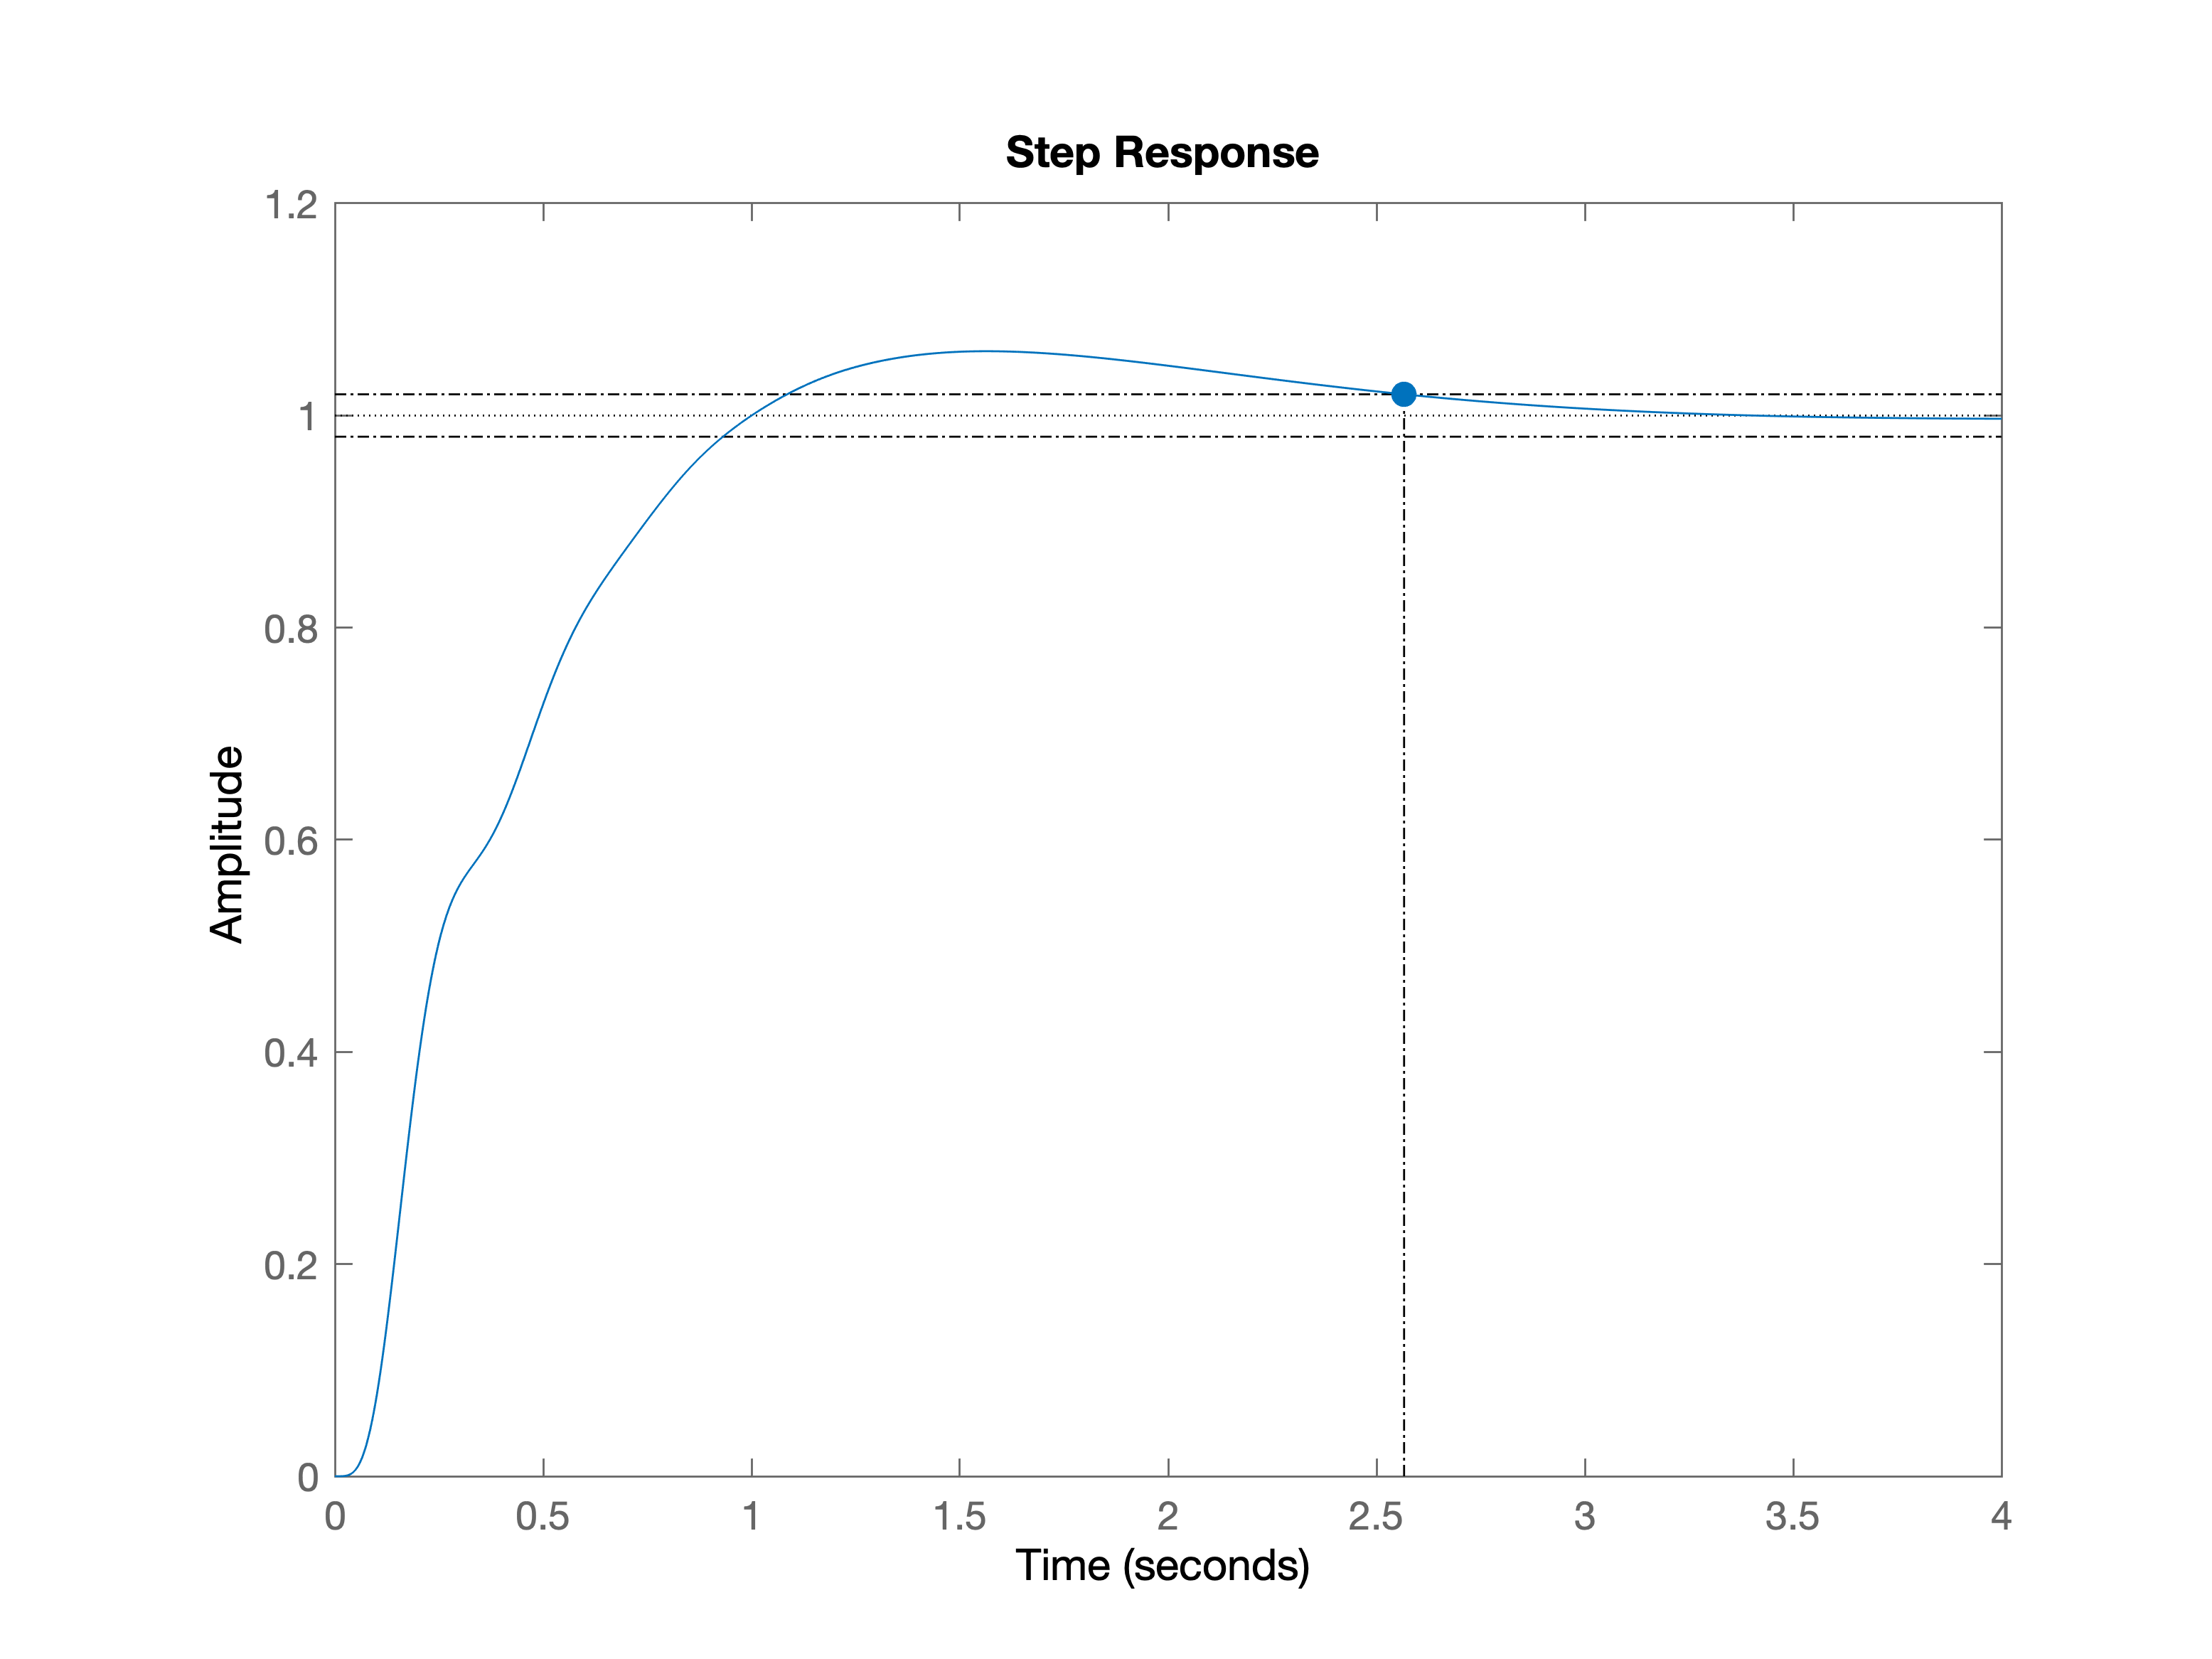
\includegraphics[width=12cm]{../Figure/P_III/chr0.png}
		\caption{پاسخ پله سیستم در حضور کنترل‌کننده PID طراحی شده \lr{CHR set point $0\%$ overshoot}}
	\end{figure}
	\item \lr{CHR set point $20\%$ overshoot}
	
	\begin{figure}[H]
		\centering
		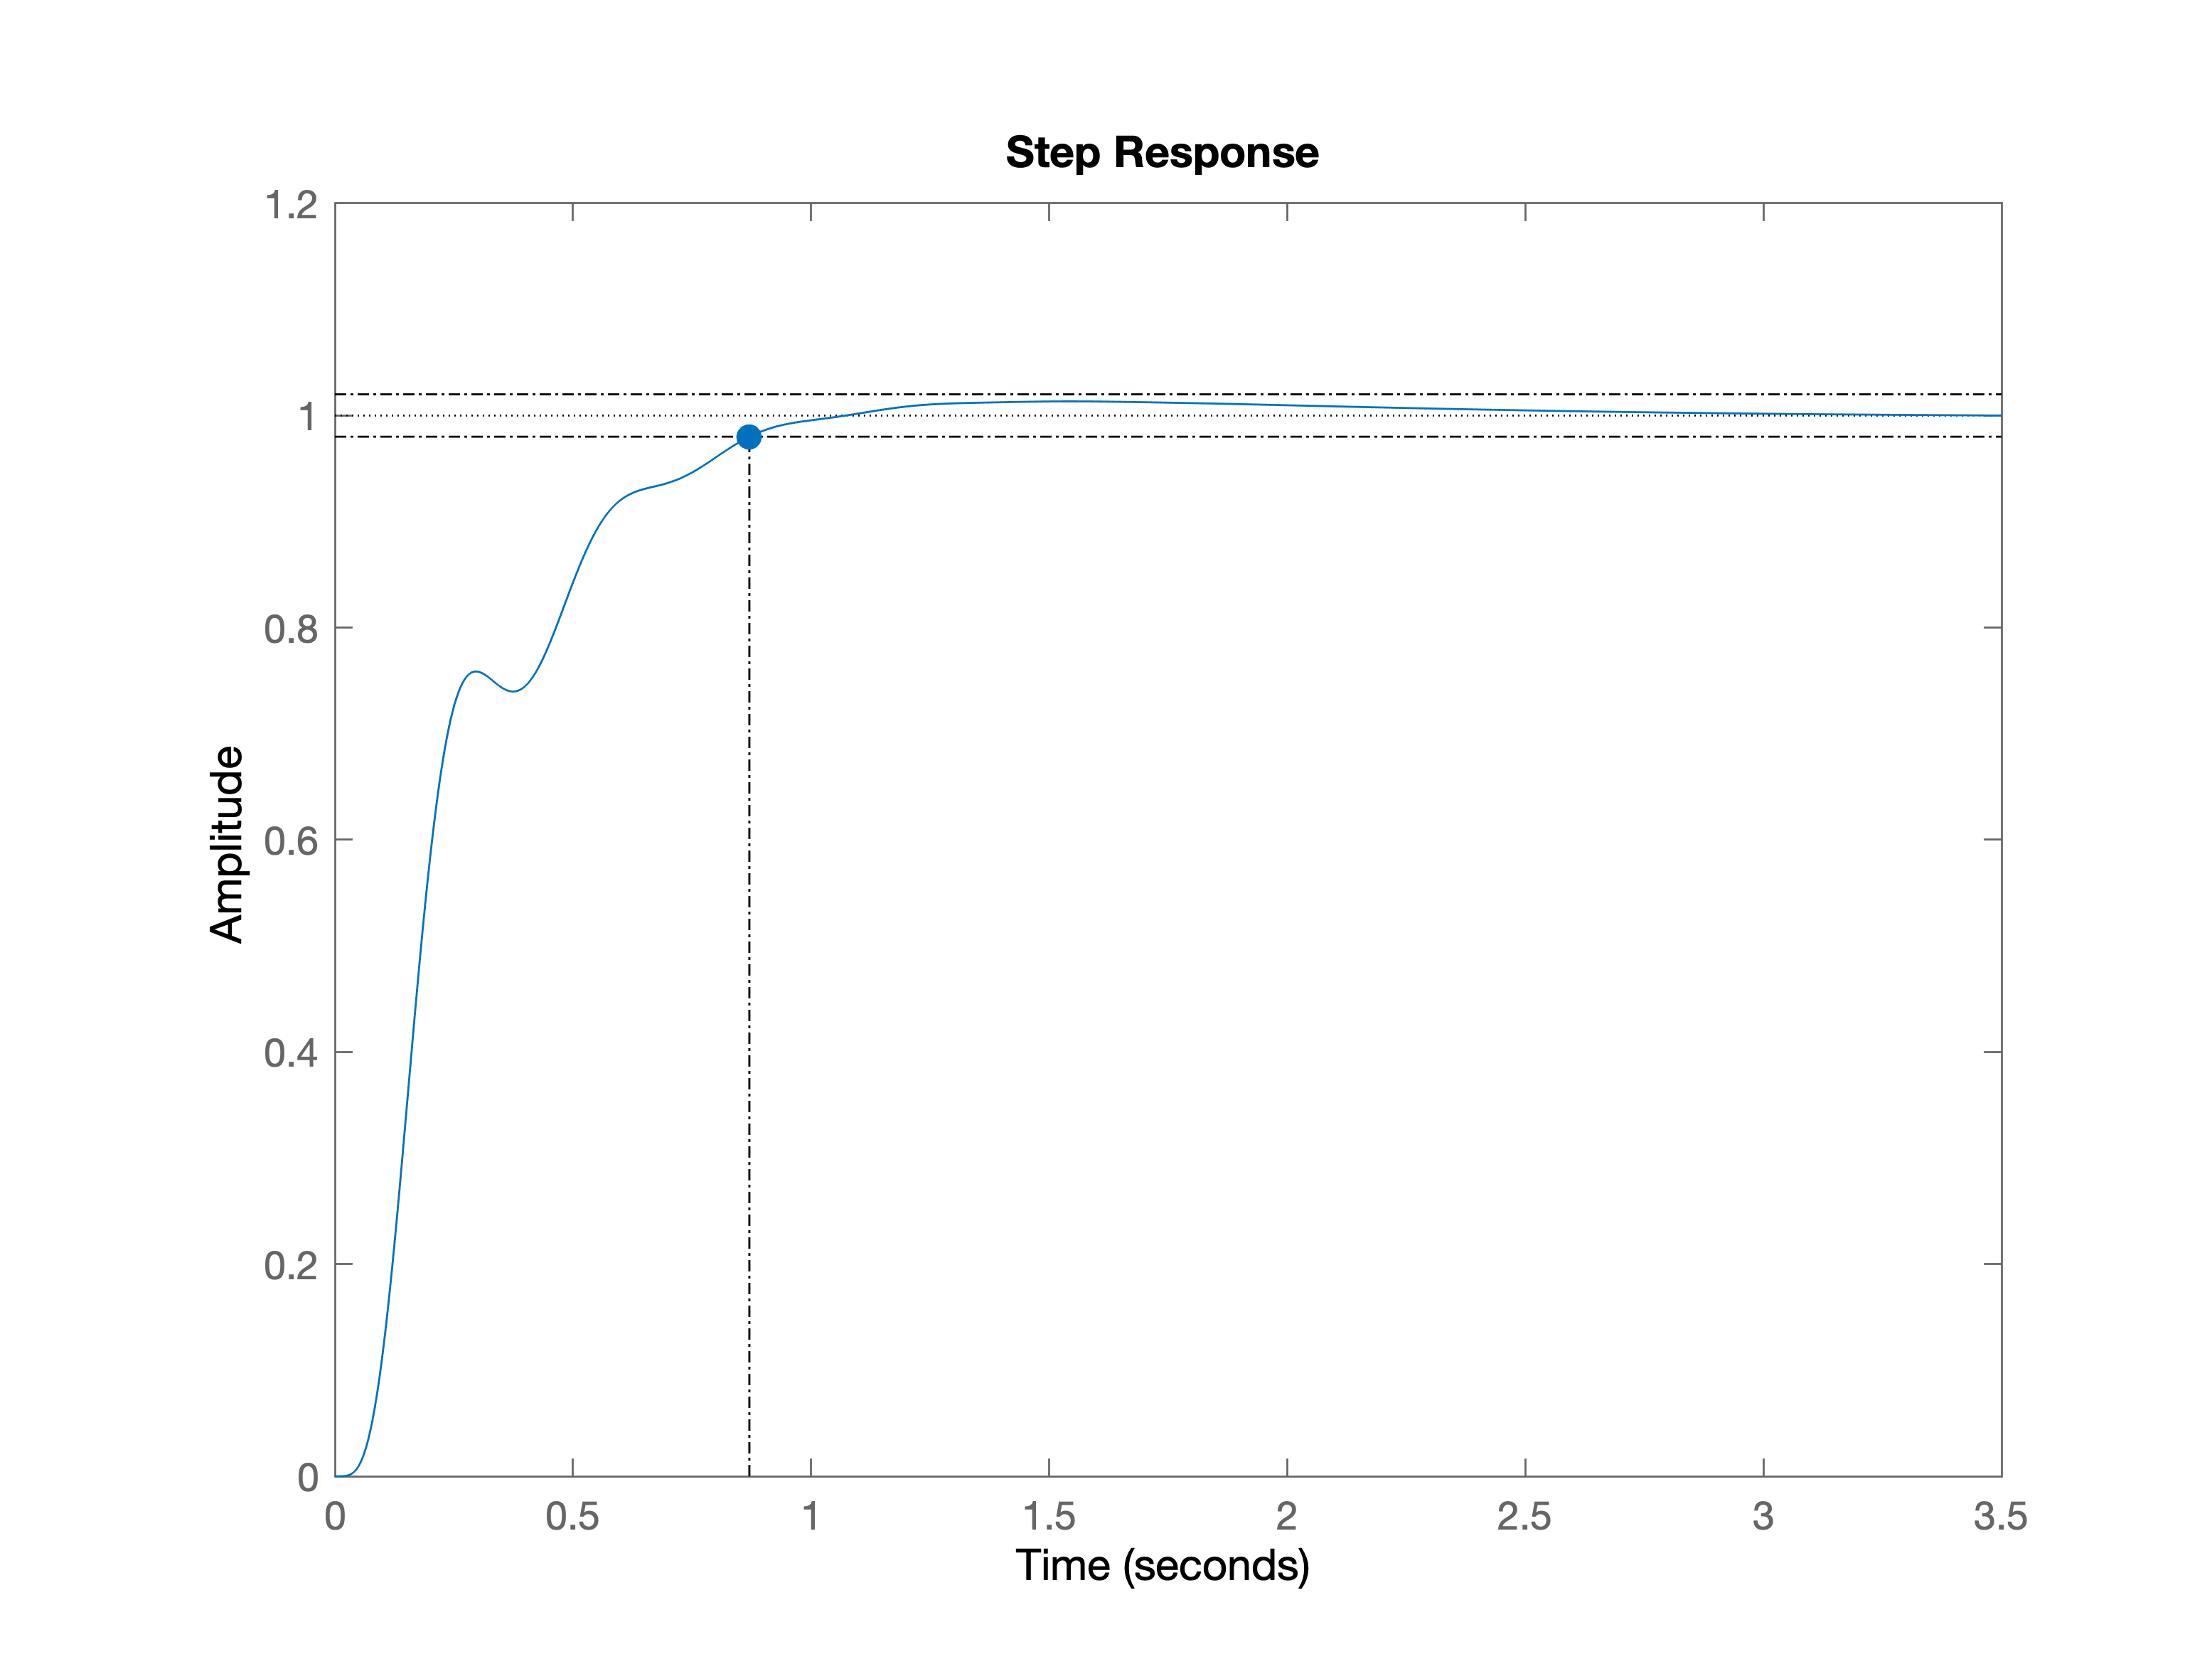
\includegraphics[width=12cm]{../Figure/P_III/chr20.png}
		\caption{پاسخ پله سیستم در حضور کنترل‌کننده PID طراحی شده \lr{CHR set point $20\%$ overshoot}}
	\end{figure}
	\item WJC
	
	\begin{figure}[H]
		\centering
		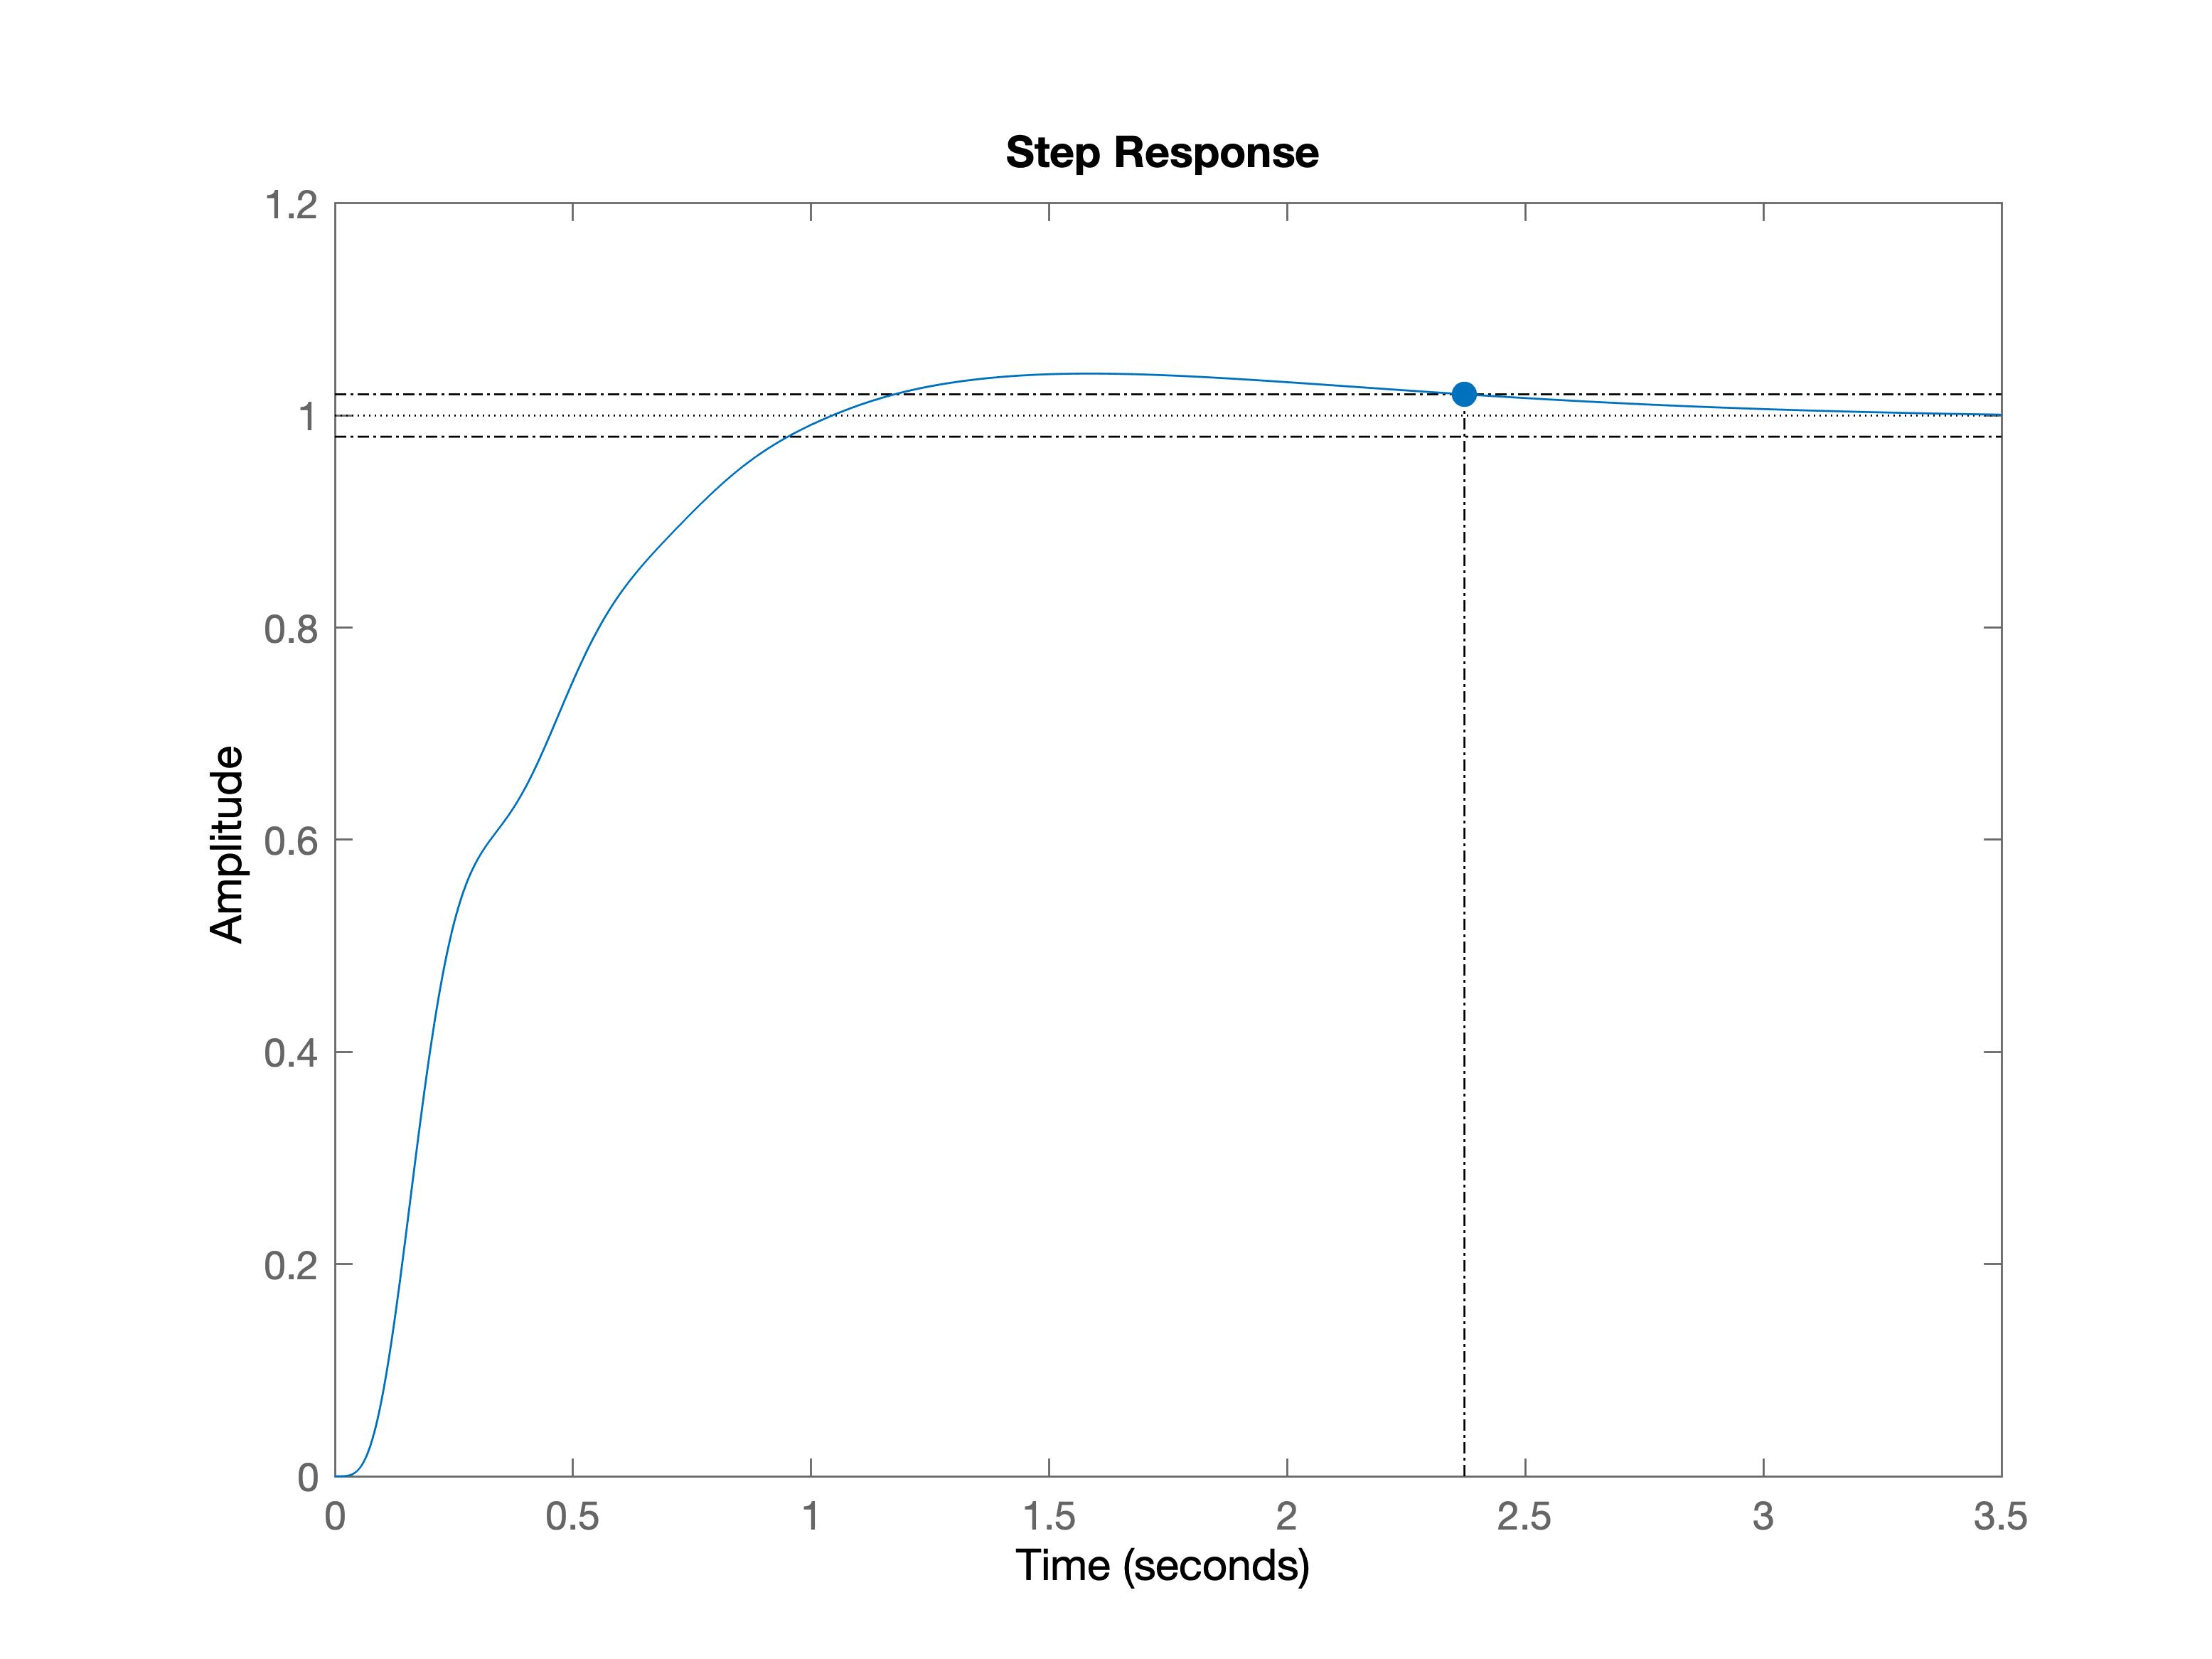
\includegraphics[width=12cm]{../Figure/P_III/wjc.png}
		\caption{پاسخ پله سیستم در حضور کنترل‌کننده PID طراحی شده \lr{WJC}}
	\end{figure}  
	\item \lr{optimum set point PID ISTE}
	
	\begin{figure}[H]
		\centering
		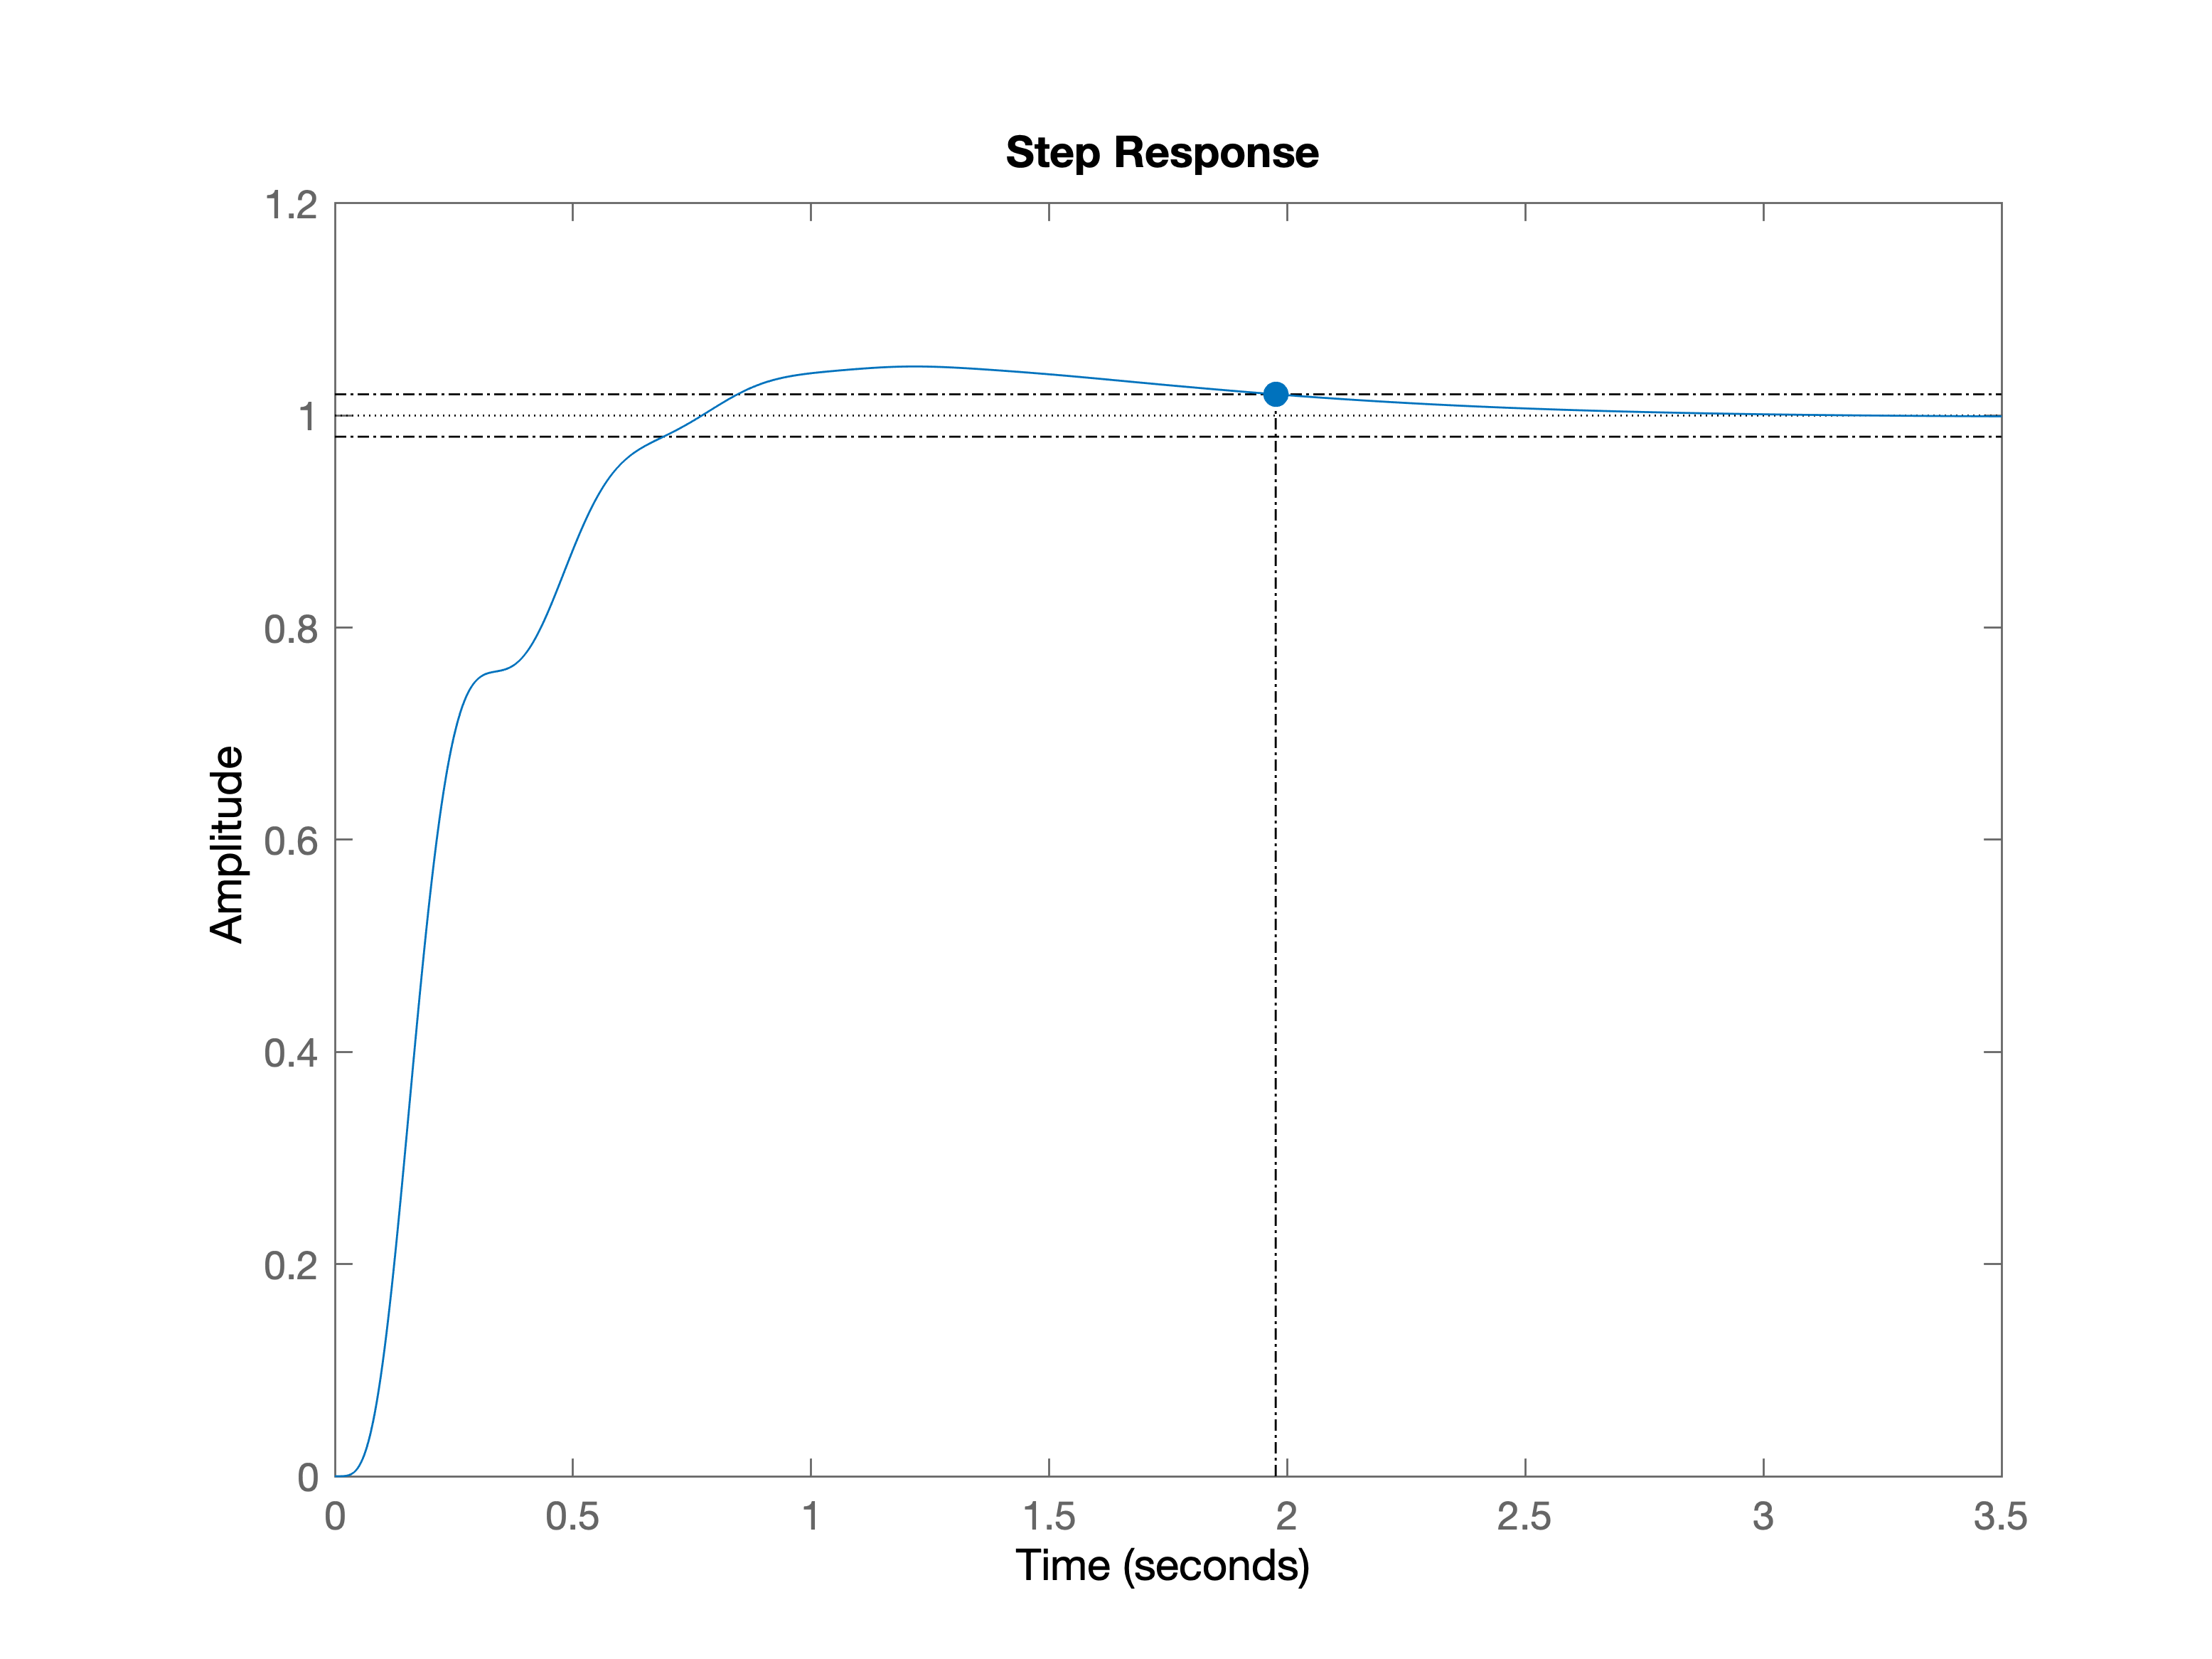
\includegraphics[width=12cm]{../Figure/P_III/optpid.png}
		\caption{پاسخ پله سیستم در حضور کنترل‌کننده PID طراحی شده \lr{optimum set point PID ISTE}}
	\end{figure}  
	\item \lr{optimum set point PI-D ISTE}
	
	\begin{figure}[H]
		\centering
		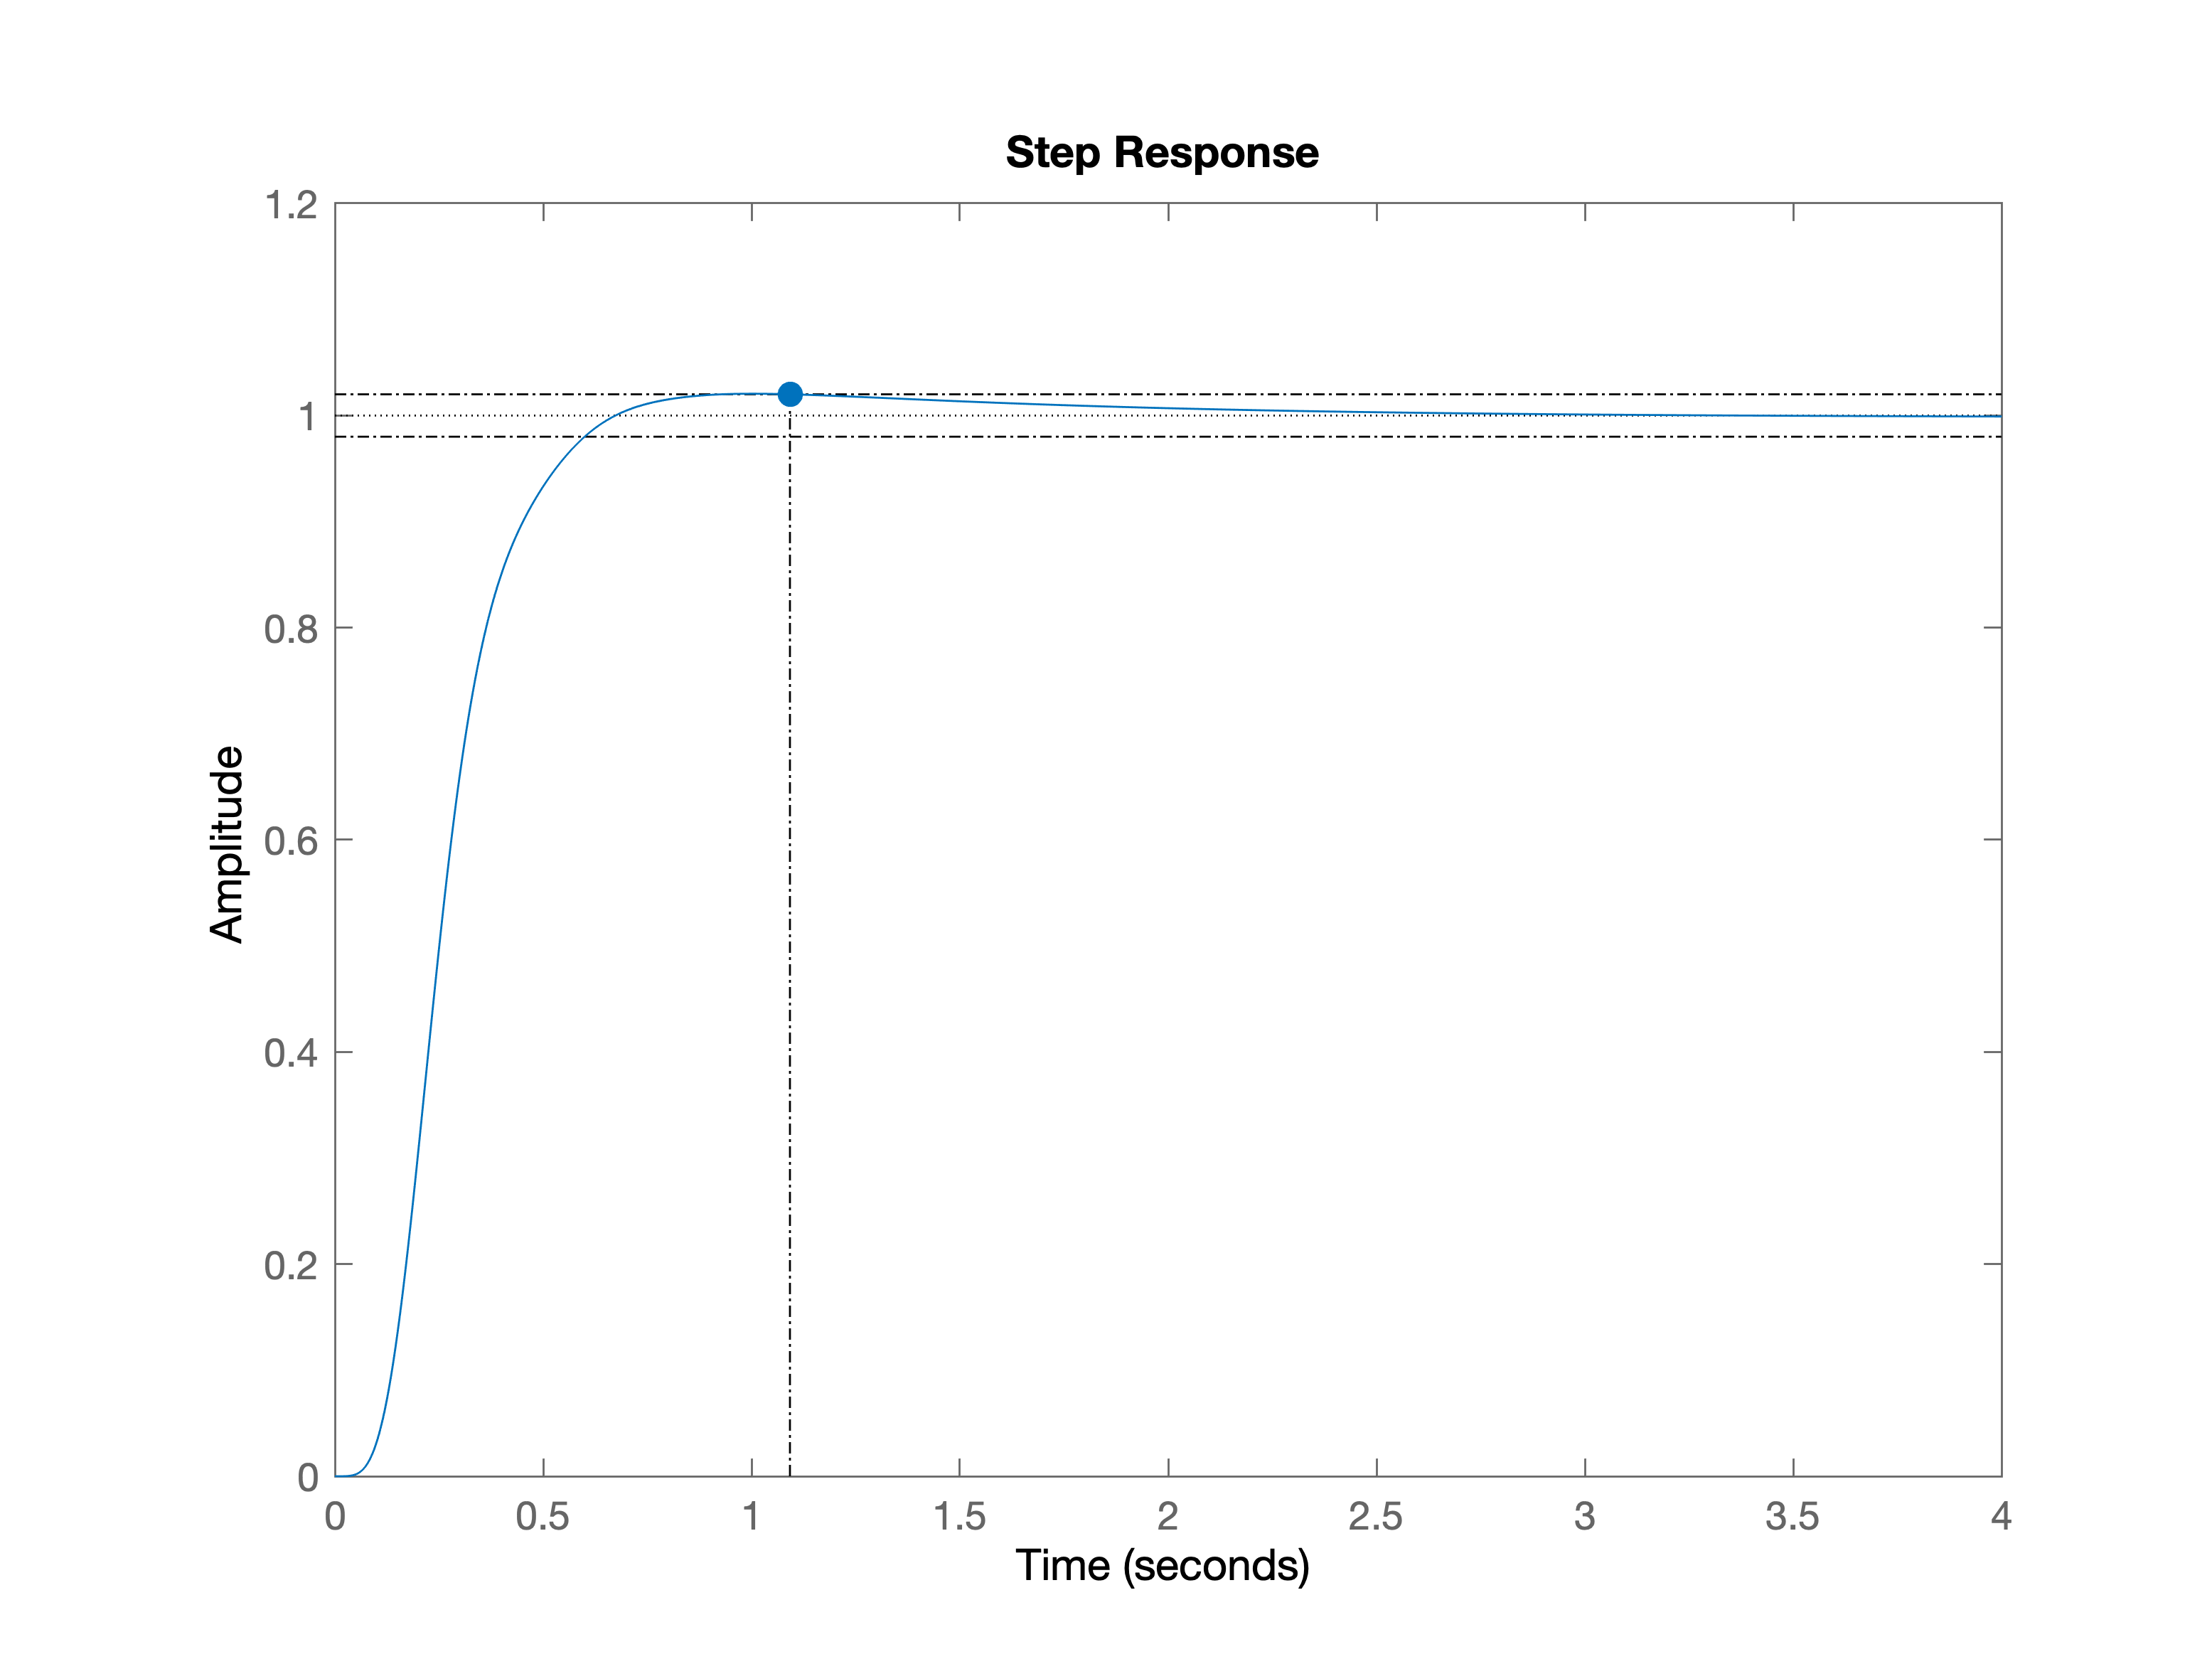
\includegraphics[width=12cm]{../Figure/P_III/optpi-d.png}
		\caption{پاسخ پله سیستم در حضور کنترل‌کننده PID طراحی شده \lr{optimum set point PI-D ISTE}}
	\end{figure}  
\end{itemize}
